%%%%%%%%%%%%%%%%%%%%%%%%%%%%%%%%%%%%%%%%%%%%%%%%%
% Spacedrive V2 Whitepaper
% Version 2.0
%%%%%%%%%%%%%%%%%%%%%%%%%%%%%%%%%%%%%%%%%%%%%%%%%
\documentclass[sigconf]{acmart}

% Code formatting packages
\usepackage{listings}
\usepackage{xcolor}
\usepackage{enumitem}
\usepackage{booktabs}
\usepackage{tikz}
\usetikzlibrary{shapes.geometric, arrows.meta, positioning, shadows, patterns, fit, backgrounds, calc}
\usepackage{pgfplots}
\usepackage{pgfplotstable} % load CSV tables
\usepackage{csvsimple} % simple CSV rendering & filtering
\usepackage{pgf-pie} % pie charts
\usepackage{subcaption} % side-by-side figures
\usepackage{siunitx} % number formatting with grouping
\pgfplotsset{compat=1.17}
\usepackage[most]{tcolorbox}

% Define colors for code highlighting
\definecolor{codegreen}{rgb}{0,0.6,0}
\definecolor{codegray}{rgb}{0.5,0.5,0.5}
\definecolor{codepurple}{rgb}{0.58,0,0.82}
\definecolor{backcolour}{rgb}{0.95,0.95,0.92}
\definecolor{keywordblue}{rgb}{0,0,0.8}

% Style for Rust code
\lstdefinestyle{ruststyle}{
 backgroundcolor=\color{backcolour},
 commentstyle=\color{codegreen},
 keywordstyle=\color{keywordblue}\bfseries,  % Add bold for keywords
 numberstyle=\tiny\color{codegray},
 stringstyle=\color{codepurple},
 basicstyle=\ttfamily\footnotesize,
 breakatwhitespace=false,
 breaklines=true,
 captionpos=b,
 keepspaces=true,
 numbers=left,
 numbersep=5pt,
 showspaces=false,
 showstringspaces=false,
 showtabs=false,
 tabsize=2,
 frame=single,
 rulecolor=\color{black!30},
 language=Rust  % Explicitly set language for highlighting
}

% Style for SQL
\lstdefinestyle{sqlstyle}{
 backgroundcolor=\color{backcolour},
 commentstyle=\color{codegreen},
 keywordstyle=\color{keywordblue},
 stringstyle=\color{codepurple},
 basicstyle=\ttfamily\footnotesize,
 numbers=left,
 numbersep=5pt,
 frame=single,
 rulecolor=\color{black!30},
 breaklines=true
}

% Style for shell/config
\lstdefinestyle{shellstyle}{
 backgroundcolor=\color{backcolour},
 commentstyle=\color{codegreen},
 basicstyle=\ttfamily\footnotesize,
 numbers=left,
 numbersep=5pt,
 frame=single,
 rulecolor=\color{black!30},
 breaklines=true
}

% Define Rust language for listings
\lstdefinelanguage{Rust}{
 keywords={
  as, async, await, break, const, continue, crate, dyn, else, enum, extern, false, fn, for, if, impl, in, let, loop, match, mod, move, mut, pub, ref, return, self, Self, static, struct, super, trait, true, type, unsafe, use, where, while
 },
 morecomment=[l]{//},
 morecomment=[s]{/*}{*/},
 morestring=[b]",
 morestring=[b]',
 sensitive=true,
}

% Define TOML language for listings
\lstdefinelanguage{toml}{
 keywords={true, false},
 morecomment=[l]{\#},
 morestring=[b]",
 morestring=[b]',
 sensitive=true,
}

% Define JSON language for listings
\lstdefinelanguage{json}{
 keywords={true, false, null},
 morestring=[b]",
 sensitive=true,
}

% Define text language for listings (simple text format)
\lstdefinelanguage{text}{
 keywords={},
 morecomment=[l]{\#},
 sensitive=false,
}

\lstset{style=ruststyle} % Set default style

% Commands for future features (marker removed)
\newcommand{\planned}[1]{#1}
\newcommand{\plannedSection}[1]{#1}

% Define Key Takeaways box environment
\tcbuselibrary{skins,breakable}
\newtcolorbox{keytakeaways}{
  enhanced,
  colback=gray!5!white,
  colframe=gray!75!white,
  boxrule=0.5pt,
  arc=2pt,
  left=12pt,
  right=12pt,
  top=10pt,
  bottom=10pt,
  before skip=10pt,
  after skip=10pt,
  breakable,
  fontupper=\small,
  before upper={\parindent=0pt\textbf{\small Key Takeaways}\par\vspace{6pt}},
  segmentation style={solid, gray!50, line width=0.3pt}
}

% --- METADATA ---
\acmConference[Spacedrive '25]{Spacedrive Whitepaper}{July 26, 2025}{Vancouver, BC, Canada}
\acmYear{2025}
\copyrightyear{2025}
\acmPrice{15.00}
\acmDOI{10.1145/nnnnnnn.nnnnnnn} % Placeholder
\acmISBN{978-x-xxxx-xxxx-x/YY/MM} % Placeholder


% --- DOCUMENT START ---
\begin{document}

% --- TITLE ---
\title{Spacedrive: Architecture of a Content-Aware Virtual File System}
\subtitle{A Local-First VDFS for Unifying Data Across Distributed Devices}

% --- AUTHORS ---
\author{James Mathew Pine}
\email{james@spacedrive.com}
\affiliation{%
\institution{Spacedrive Technology Inc.}
\city{Vancouver}
\state{British Columbia}
\country{Canada}
}

% --- ABSTRACT ---
\begin{abstract}
Data fragmentation across devices and clouds hinders cohesive file management. Spacedrive implements a local-first~\cite{kleppmann_localfirst_2019} Virtual Distributed File System (VDFS) that unifies data views while preserving original file locations. Unlike cloud-centric alternatives, it supports offline operation, minimizes reliance on centralized services, and is applicable to both single-user and organizational deployments.

Core features include a unified data index for low-latency search, content-aware deduplication, and transactional cross-device operations. This index also supports a local AI component for natural language queries and assistive automation.

This paper describes the Spacedrive v2 architecture, including content-aware addressing, transactional previews, and a hybrid synchronization model that avoids distributed consensus by combining simple state-replication for device-authoritative data with a lightweight, HLC-ordered log for shared metadata. The Content Identity system enables deduplication and redundancy tracking, while AI integration provides semantic search and optional automated actions. We also present a cloud deployment in which backends participate as standard P2P devices, reducing client–server asymmetry.
\end{abstract}


% --- KEYWORDS & CCS ---
\begin{CCSXML}
<ccs2012>
<concept>
 <concept_id>10002951.10003152.10003153.10003155</concept_id>
 <concept_desc>Information systems~Hierarchical storage management</concept_desc>
 <concept_significance>500</concept_significance>
</concept>
<concept>
 <concept_id>10002951.10003317.10003325.10003326</concept_id>
 <concept_desc>Information systems~Query representation</concept_desc>
 <concept_significance>500</concept_significance>
</concept>
<concept>
 <concept_id>10011007.10011006.10011072</concept_id>
 <concept_desc>Software and its engineering~Software architectures</concept_desc>
 <concept_significance>500</concept_significance>
</concept>
</ccs2012>
\end{CCSXML}

\ccsdesc[500]{Information systems~Hierarchical storage management}
\ccsdesc[500]{Information systems~Query representation}
\ccsdesc[500]{Software and its engineering~Software architectures}

\keywords{Virtual Distributed File System, VDFS, AI-Native Architecture, Natural Language File Management, Semantic Search, Data Synchronization, Tiered Storage, Local-First AI, Rust}

\maketitle

% --- SECTION 1: INTRODUCTION ---
\section{Introduction}

The proliferation of computing devices and cloud services has fragmented our digital lives, scattering assets across incompatible ecosystems~\cite{bergman_fragmentation_2006, atlassian2025}. Knowledge workers waste up to 25\% of their time searching for files, with creative professionals particularly affected~\cite{atlassian2025}. Existing solutions force a choice between cloud convenience and local control, with none offering a unified, content-aware approach.

Spacedrive addresses this by implementing a \textbf{local-first Virtual Distributed File System (VDFS)} that unifies data management while files remain in their original locations~\cite{kleppmann_localfirst_2019}. Unlike cloud-centric services, it supports offline operation, preserves local control, and applies to both single-user and multi-user deployments.

The architecture is built on four foundational principles that solve traditionally hard problems in distributed systems:

\begin{itemize}[noitemsep, topsep=0pt]
 \item \textbf{Unified Data Model: The Content-Aware VDFS} (Section~\ref{sec:vdfs}): A single, virtual layer that unifies all data across devices by focusing on the content of files, not just their names and locations. Built on an Entry-Centric Model (Section~\ref{sec:entry-centric}) where every file and folder is a first-class object capable of holding rich metadata instantly, and a Content Identity System (Section~\ref{sec:content-identity}) that uses adaptive hashing to identify and track unique file content, enabling deduplication, redundancy tracking, and resilient content-based addressing.

 \item \textbf{Safe \& Predictable Operations: The Transactional Action System} (Section~\ref{sec:action-system}): A system designed to make file operations safe and transparent. Every change to the VDFS is treated as a transaction that is simulated and approved before execution, leveraging the complete VDFS index to run in-memory simulations of proposed actions with previews of outcomes, including conflicts or storage issues.

 \item \textbf{Resilient Synchronization: A Leaderless Hybrid Model} (Section~\ref{sec:library-sync}): A synchronization model that eliminates leader-based bottlenecks by separating data into distinct domains. The filesystem index, being device-authoritative, is replicated across all devices, enabling File Sync to operate through efficient index queries rather than filesystem scanning. Concurrently modified user metadata is merged deterministically using a lightweight, per-device change log ordered by a Hybrid Logical Clock (HLC).

 \item \textbf{AI Agent Architecture} (Section~\ref{sec:ai-native}): An architecture where specialized AI agents are implemented as WASM extensions, each with domain-specific knowledge and persistent memory systems. These agents observe the VDFS index, react to events, and propose actions using the same transactional model as human-initiated operations.
\end{itemize}

We report a reference implementation in Rust. On consumer hardware, we observe sub-100 ms semantic search latency, synchronization via the Iroh networking stack, and an approximate memory footprint of 150 MB for libraries exceeding one million files.

This paper details Spacedrive's architecture as a production system implemented in Rust. We show how domain separation and content awareness enable cross-device deduplication, semantic search, storage tiering, and synchronization without distributed consensus.

Spacedrive adapts to mobile device constraints through built-in resource management. On battery power, it reduces CPU usage. It respects data limits and platform background restrictions. The system runs efficiently on both desktops and smartphones, maintaining performance across all devices.

Spacedrive applies local-first architecture~\cite{kleppmann_localfirst_2019} principles at scale. Traditional enterprise systems sacrifice user experience for control. Consumer tools lack business security features. Spacedrive aims to provide both. It scales from personal use to enterprise deployment while maintaining security, data sovereignty, and compliance.

We also outline a cloud service built on this architecture. The cloud backend runs as a standard Spacedrive device. Users pair with it using the same peer-to-peer protocols as local machines. This hybrid approach offers cloud-hosted availability while retaining local-first privacy and control properties.


% --- SECTION 2: RELATED WORK ---
\section{Related Work}
Spacedrive builds upon decades of research in distributed file systems, personal information management, and content-addressable storage~\cite{quinlan_venti_2002}. We position our work within this landscape to highlight our unique contributions.

\subsection{Traditional Cloud Sync Services}
Commercial cloud storage services (Dropbox~\cite{dropbox}, Google Drive, iCloud) provide basic file synchronization but suffer from platform lock-in and lack content-addressing. These services treat files as opaque blobs, missing opportunities for deduplication and semantic understanding. Unlike Spacedrive, they require continuous internet connectivity and centralize user data on corporate servers.

\subsection{Distributed File Systems}
Research systems like IPFS~\cite{ipfs} and production systems like Ceph~\cite{ceph} demonstrate the power of content-addressable storage. However, their complexity and resource requirements make them unsuitable for personal use. IPFS requires understanding of cryptographic hashes and peer-to-peer networking, while Ceph targets datacenter deployments. Spacedrive adopts content-addressing principles while hiding complexity behind familiar file management interfaces, drawing inspiration from systems like LBFS~\cite{muthitacharoen_lbfs_2001} that pioneered content-defined chunking for efficient network transfers.

\subsection{Virtual Distributed File Systems in the Datacenter}
The concept of a Virtual Distributed File System (VDFS) has been explored in the context of large-scale data analytics. Alluxio (formerly Tachyon)~\cite{alluxio_vdfs} introduced a memory-centric VDFS designed to sit between computation frameworks like Apache Spark and various storage systems (e.g., HDFS, S3). Alluxio's primary goal is to accelerate data analytics jobs by providing a consolidated, high-throughput data access layer, effectively decoupling computation from storage in a datacenter environment.

While Spacedrive shares the VDFS terminology, its architectural goals and target domain are fundamentally different. Where Alluxio optimizes for performance in large, multi-tenant analytics clusters, Spacedrive is designed as a local-first, privacy-preserving data space for an individual's complete digital life. Spacedrive's innovations in universal addressing (\texttt{SdPath}), an entry-centric model with immediate metadata, and Library Sync are tailored to the challenges of personal data fragmentation across a heterogeneous collection of consumer devices, a problem space distinct from the performance and data-sharing challenges in large-scale analytics that Alluxio addresses.

\subsection{Personal Knowledge Management}
Tools like Obsidian and Logseq excel at managing structured knowledge through markdown files but lack general file management capabilities. They demonstrate the value of local-first architectures~\cite{kleppmann_localfirst_2019} and portable data formats, principles that Spacedrive extends to all file types. Our work generalizes their approach from text-centric knowledge graphs to general-purpose file management.

\subsection{Self-Hosted Solutions}
Projects like Nextcloud provide self-hosted alternatives to commercial cloud services but retain client-server architectures that complicate deployment and maintenance. They require dedicated servers and technical expertise, limiting adoption. Spacedrive's peer-to-peer architecture eliminates server requirements while providing similar capabilities through direct device communication.

\subsection{Semantic File Systems}
Academic projects exploring semantic file organization date back to the Semantic File System~\cite{gifford_sfs_1991} and Presto~\cite{dourish_presto_1999}. While these demonstrated the value of content-based organization, they predated modern AI capabilities. Spacedrive applies contemporary machine learning, enabling natural language queries and automated tasks that were not feasible in earlier systems.

\subsection{Comparative Analysis}

Table~\ref{tab:comparison} summarizes how Spacedrive advances beyond existing systems by combining their strengths while addressing their limitations.

\begin{table*}[ht]
\centering
\footnotesize
\setlength{\tabcolsep}{4pt}
\begin{tabular}{@{}p{2.2cm}p{2.5cm}p{2cm}p{2.5cm}p{4.5cm}p{2.3cm}@{}}
\toprule
\textbf{System} & \textbf{Architecture} & \textbf{Target Users} & \textbf{Key Innovation} & \textbf{Primary Limitation} & \textbf{Privacy Model} \\
\midrule
Dropbox/\newline iCloud & Client-Server & Consumers & Simple sync & No content addressing, vendor lock-in & Cloud-\newline centralized \\
IPFS & P2P DHT & Developers & Content addressing & Complex for consumers, no AI & Public by default \\
Ceph & Distributed cluster & Enterprises & Scalable storage & Datacenter-focused, high overhead & Configurable \\
Alluxio & Memory-centric VDFS & Analytics teams & Unified data access & Not for personal files & Enterprise-\newline managed \\
Nextcloud & Self-hosted server & Tech-savvy users & Data sovereignty & Requires dedicated server & Self-hosted private \\
\textbf{Spacedrive} & \textbf{Local-first P2P} & \textbf{Everyone} & \textbf{AI-native VDFS} & \textbf{Higher resource usage than simple browsers} & \textbf{Local-first E2E} \\
\bottomrule
\end{tabular}
\caption{Comparison of Spacedrive with existing systems, expanded with privacy models for completeness.}
\label{tab:comparison}
\end{table*}

Our work synthesizes insights from these domains while addressing their individual limitations, creating an integrated system that is effective, private, and accessible to non-technical users.

\subsection{Command-Line Data Movers}
Command-line utilities like rclone~\cite{rclone_reference} excel at performing scriptable data transfers between a wide variety of storage backends. These tools are effective for one-off data moving tasks and are a staple for technical users. However, their fundamentally stateless architecture presents limitations that Spacedrive's stateful, persistent model addresses.

Each time a command is executed, a stateless tool must re-query both the source and destination to determine the necessary changes. Spacedrive, in contrast, operates as a data orchestrator rather than just a data mover. It maintains a continuously updated VDFS index, enabling it to know the state of files across locations in real time. Spacedrive leverages its persistent state to perform synchronization through global content-aware deduplication, optimal path routing for transfers, and a "preview-then-commit" transactional model that enhances safety and reliability. While rclone is a widely used tool for explicit data transfer, Spacedrive operates at a higher level of abstraction, integrating synchronization as a native, persistent feature of a cohesive data space. The system's approach to maintaining index integrity during offline periods is detailed in Section~\ref{sec:offline-recovery}.
\paragraph{Extensibility Models}
Unlike systems that require native plugins (Finder, Nautilus) or rely on scripting languages (Obsidian, VS Code), Spacedrive employs a consistent WebAssembly-based extensibility model. All extensions—from simple content type handlers to complex cloud storage integrations—run in a secure WASM sandbox. This provides both power and safety without the complexity of managing multiple extension systems.

\paragraph{Cloud Storage Approaches}
Unlike traditional sync clients that duplicate data locally, Spacedrive treats cloud storage as just another volume through direct indexing (detailed in Section~\ref{sec:platform-integrations}, including traditional protocols like FTP and SMB).

% --- SECTION 3: LEARNING FROM THE PAST ---
\section{Learning from the Past: Architectural Evolution from Spacedrive v1}

Spacedrive v2 represents a complete architectural reimplementation designed to fulfill the original vision on a more reliable and scalable foundation. The initial version, first open-sourced in 2022, validated the core premise of an integrated VDFS for personal data with significant community interest. However, as development progressed through early 2025, several foundational architectural challenges emerged that ultimately necessitated this rewrite, drawing lessons from the evolution of distributed systems and CRDTs~\cite{shapiro_crdts_2011}.

\subsection{Key Challenges in the Original Architecture}

The development of v1 provided invaluable insights that shaped the v2 architecture. Building Spacedrive required pioneering work in an immature ecosystem—Rust application development was uncommon at the time, Tauri was in its infancy, and many essential libraries simply didn't exist. Our engineers contributed extensively upstream to Tauri, Iroh, and even the QUIC protocol, with Spacedrive serving as a real-world model for building complex Rust applications. We developed critical infrastructure including prisma-client-rust and rspc, which became foundational tools for the broader Rust ecosystem. However, this pioneering approach created architectural challenges: separate systems for indexed and non-indexed files that couldn't interoperate, tight frontend/backend coupling through query invalidation patterns, and the complexity overhead of custom CRDT-based synchronization. The experience highlighted the importance of unified addressing systems, streamlined job architectures, and the risks of maintaining custom infrastructure when mature alternatives emerge.

\subsection{Spacedrive v2 as an Architectural Solution}

The v2 architecture directly addresses these challenges. The universal \textbf{SdPath} addressing system eliminates the dual file system problem entirely. A decoupled \textbf{Event Bus} provides reliable state propagation, and a simpler domain-separated \textbf{Library Sync} model ensures consistency without CRDT complexity by employing a leaderless, hybrid architecture. This model uses efficient state-based replication for device-authoritative data and a lightweight, HLC-ordered log for shared metadata, eliminating single points of failure. The new job system reduces boilerplate by over 90\%, while a consolidated networking layer powered by \textbf{Iroh} unifies all P2P communication, improving reliability and connection performance~\cite{iroh_networking}. The technology stack was also modernized, replacing abandoned libraries with community-trusted alternatives like \textbf{SeaORM}.

By learning from real-world challenges of the initial version, Spacedrive v2 delivers on the original promise with an architecture that is simpler, more fault-tolerant, and designed for the long term.

\paragraph{Extensibility Lessons}
Version 1's monolithic architecture limited community contributions. Version 2's single WASM plugin model enables an active ecosystem while maintaining security and stability. All extensions—from content type handlers to cloud storage providers—run in the same secure sandbox, simplifying development and distribution.


% --- SECTION 4: THE SPACEDRIVE ARCHITECTURE ---
\section{The Spacedrive Architecture}
\label{sec:architecture}

\begin{keytakeaways}
\begin{itemize}[noitemsep, topsep=0pt]
\item \textbf{Core Innovation}: Integrated virtual layer that makes distributed storage feel like a single filesystem through content-aware addressing
\item \textbf{Key Components}: VDFS model with SdPath addressing • Entry-centric metadata • Content Identity deduplication • Transactional Actions • AI-native design
\item \textbf{Design Philosophy}: Local-first for privacy, peer-to-peer for resilience, AI-assisted analysis---while preserving user control
\end{itemize}
\end{keytakeaways}

Spacedrive's architecture represents a new approach to how personal data is managed across devices. Rather than treating files as isolated entities scattered across different storage systems, Spacedrive creates a cohesive virtual layer that provides consistent access, metadata and analysis, and cross-device synchronization. This section presents the core architectural components that enable this vision.

\begin{figure*}[!ht]
    \centering
    \includegraphics[width=\textwidth]{architecture.png}
    \caption{Spacedrive System Architecture}
    \label{fig:architecture}

    \vspace{0.5em}
    \small
    The provided figure illustrates the Spacedrive system architecture, a modular design centered around the \textbf{Spacedrive Core (VDFS Engine)}. A user is looking at the flow of a command as it originates from clients or automated systems like the AI Engine. The command is processed by the \textbf{Transactional Action System} for validation, then dispatched to the \textbf{Durable Job System} for execution. These jobs, which range from content indexing to file synchronization, interact with data via a \textbf{Unified File System} that sits above physical storage. The final state, including the file index and any extracted metadata, is maintained in the \textbf{Spacedrive Library}, which serves as the persistent state of the system.
\end{figure*}

% --- SECTION 4.1: THE VDFS MODEL ---
\subsection{The VDFS Model}
\label{sec:vdfs}
At the core of Spacedrive is a set of abstractions that model a user's data not as a collection of disparate file paths, but as a cohesive, integrated Library with content-aware relationships.

\subsubsection{The Library: A Portable Data Container}
Rather than managing scattered databases and configurations, Spacedrive organizes everything into self-contained \textbf{Libraries}. Each Library is a \texttt{.sdlibrary} directory that functions as a complete, portable data container:


A Spacedrive Library is organized as a self-contained directory with four key components:

\begin{itemize}[noitemsep, topsep=0pt]
 \item \textbf{Configuration File}: Library settings and device registry
 \item \textbf{Metadata Database}: Complete file index with relationships and tags
 \item \textbf{Thumbnail Cache}: Organized storage for instant previews
 \item \textbf{Concurrency Protection}: Safe multi-device access control
\end{itemize}

This portable structure means that backing up your entire organizational system—all metadata, tags, and file relationships—is as simple as copying a single directory. The Library acts as a complete catalog of your digital life, preserving your organizational work even if the actual files are distributed across multiple devices and locations.

This design provides several critical advantages: its self-contained nature simplifies backup and migration, and sharing involves sending the complete Library. From a security perspective, this architecture ensures that each device in a paired group builds and controls its own library database, enabling granular scoping of locations and indexed data to local or select devices, thereby enhancing data sovereignty and limiting exposure.

\subsubsection{The Entry-Centric Data Model}
\label{sec:entry-centric}
The fundamental unit within a Library is the \textbf{Entry}---a universal representation that treats files and directories as first-class, queryable objects. This design, building upon early work in document-centric computing~\cite{dourish_presto_1999}, enables the VDFS to maintain rich metadata and relationships independently of the underlying filesystem.

\textbf{Uniform Representation}: Unlike traditional filesystems where directories and files have fundamentally different representations, every filesystem entity becomes an Entry with consistent properties:

\begin{table}[h]
\footnotesize
\centering
\begin{tabular}{@{}ll@{}}
\toprule
\textbf{Field} & \textbf{Purpose} \\
\midrule
Unique ID & Globally unique, immutable identifier \\
Universal Path & Complete location addressing (SdPath) \\
Parent ID & Direct hierarchical relationship \\
Metadata ID & Links to user-assigned metadata \\
Content ID & Links to content identity (for deduplication) \\
Discovery Time & Temporal tracking \\
\bottomrule
\end{tabular}
\caption{Entry data model}
\label{tab:entry-fields}
\end{table}

\textbf{Architectural Benefits}: This entry-centric approach provides several key advantages:

\begin{itemize}[noitemsep, topsep=0pt]
 \item \textbf{Metadata Independence}: User metadata (tags, notes) persists regardless of filesystem changes. Moving or renaming files preserves all organizational work.

 \item \textbf{Universal Queryability}: Every entity can be searched, filtered, and organized through the same query interface, whether it's a file, directory, or even ephemeral content.

 \item \textbf{Relationship Tracking}: The parent ID creates an explicit graph structure that enables O(1) hierarchical queries through the closure table (Section~\ref{sec:indexing-engine}), replacing slow path-based traversals.

 \item \textbf{Content Separation}: The optional content ID links entries to the deduplication system without coupling file identity to content analysis. An entry can exist and be organized before its content is analyzed.
\end{itemize}

\textbf{Ephemeral Mode}: The indexing engine extends this model to support temporary, in-memory Entry records for unindexed content. When browsing external drives or remote devices, ephemeral entries are generated on-the-fly and presented alongside persisted entries, creating a unified view. Users can tag and organize these files immediately; if an entry lacks a parent Location, it persists in the Library with its metadata intact, demonstrating how the entry-centric model handles both permanent and transient data uniformly.

\subsubsection{Semantic Tagging}
Spacedrive employs a graph-based tagging system that supports semantic organization while maintaining ease of use. This system recognizes that human organization relies on context, relationships, and multiple perspectives---capabilities that traditional flat tagging systems cannot provide.

\textbf{Contextual Tag Design}

The tagging system provides flexibility:

\begin{itemize}[noitemsep, topsep=0pt]
 \item \textbf{Polymorphic Naming}: Tags embrace natural ambiguity, allowing multiple "Project" tags differentiated by their semantic context rather than forced uniqueness
 \item \textbf{Unicode-Native}: Full international character support enables native-language organization without ASCII constraints
 \item \textbf{Semantic Variants}: Each tag maintains multiple access points---formal names, abbreviations, and contextual aliases
\end{itemize}

\textbf{Graph-Based Organization Model}

The system implements a directed acyclic graph (DAG) structure using optimized database patterns for millisecond-scale hierarchy traversal:

\textbf{Context Resolution}: When multiple tags share names, the system resolves ambiguity through relationship analysis. A "Phoenix" tag might represent a city under "Geography" or a mythical creature under "Mythology", with automatic contextual display based on the tag's position in the semantic graph.

\textbf{Organizational Benefits}:
\begin{itemize}[noitemsep, topsep=0pt]
 \item \textbf{Implicit Classification}: Tagging a document with "Quarterly Report" automatically inherits organizational context from "Business Documents" and "Financial Records"
 \item \textbf{Semantic Discovery}: Queries for "Corporate Materials" surface all descendant content through graph traversal
 \item \textbf{Emergent Patterns}: The system surfaces inferred organizational connections
\end{itemize}

\textbf{Advanced Tag Capabilities}

Beyond basic labeling, tags function as rich metadata objects:

\begin{itemize}[noitemsep, topsep=0pt]
 \item \textbf{Organizational Roles}: Tags marked as organizational anchors create visual hierarchies in the interface
 \item \textbf{Privacy Controls}: Archive-style tags can shield content from standard searches while maintaining accessibility
 \item \textbf{Visual Semantics}: Customizable appearance properties encode meaning through color and iconography
 \item \textbf{Compositional Attributes}: Support attribute composition (e.g., "Technical Document" WITH "Confidential" AND "2024 Q3")
\end{itemize}

This architecture treats tags as first-class metadata that capture relationships in personal data organization, scaling from basic keyword tagging to organizational knowledge management.

\subsubsection{SdPath: Universal File Addressing}
Central to the VDFS abstraction is \textbf{SdPath}---a universal addressing system that makes device boundaries transparent. While the primary form provides a direct physical coordinate (device identifier + local path), Spacedrive also supports a content-aware addressing mode that transforms SdPath from a simple pointer into a content resolver.

\begin{lstlisting}[language=Rust, caption={SdPath supports both physical and content-aware addressing}]
#[derive(Clone, Debug)]
pub enum SdPath {
    // Physical addressing: device + path
    Physical {
        device_id: DeviceId,
        local_path: PathBuf
    },
    // Cloud addressing: cloud volume + path
    Cloud {
        volume_id: Uuid,
        path: String  // Cloud-native path format
    },
    // Content-aware addressing: find optimal instance
    Content {
        content_id: Uuid
    },
}
\end{lstlisting}

\textbf{Content-Aware Addressing and Optimal Path Resolution}

Content-aware addressing allows Spacedrive to automatically find the best available copy of a file across all devices. Instead of failing when a specific device is offline, the system automatically locates and uses alternative copies---turning device-specific file paths into content handles that continue to function.

When an operation is initiated with a content-aware \texttt{SdPath}, Spacedrive performs an \textbf{optimal path resolution} query against the Library index:

\begin{enumerate}[noitemsep, topsep=0pt]
    \item \textbf{Content Lookup}: Query the \texttt{Content Identity} table to find all instances of the file content across all devices

    \item \textbf{Candidate Evaluation}: Evaluate each instance based on a cost function considering:
    \begin{itemize}[noitemsep]
        \item \textbf{Locality}: Local device copies prioritized above all others
        \item \textbf{Network Proximity}: Iroh provides real-time latency and bandwidth estimates
        \item \textbf{Device Availability}: Filter for currently online devices
        \item \textbf{Storage Tier}: Volume-Aware Storage Foundation prioritizes SSD over HDD
    \end{itemize}

    \item \textbf{Path Selection}: Select the lowest-cost valid path and proceed transparently
\end{enumerate}

This mechanism makes file operations more resilient. If a user requests a file from an offline laptop, Spacedrive can source the identical content from a NAS on the local network. This elevates \texttt{SdPath} from a simple address to an abstract, location-independent handle for content.

\textbf{Practical Applications}

This addressing system enables operations that were previously impossible or extremely complex:

\begin{itemize}[noitemsep, topsep=0pt]
 \item \textbf{Availability-Aware Operations}: File operations can succeed even when the original source is offline
 \item \textbf{Performance-Aware Source Selection}: Automatically select the fastest available source
 \item \textbf{Simplified Development}: Applications reference content by ID without managing device availability
 \item \textbf{Automatic Failover}: Operations automatically switch to alternative sources
\end{itemize}

This abstraction simplifies cross-device operations into type-safe function calls. The distributed filesystem appears local to users and developers.

\paragraph{Universal URI Scheme}
To make these addressing modes accessible and ergonomic for clients, APIs, and command-line interfaces, Spacedrive establishes a unified string-based URI scheme. This allows any path, whether physical or content-based, to be represented as a simple, standardized string:
\begin{itemize}[noitemsep, topsep=0pt]
    \item \textbf{Physical Path}: A physical location is represented as \texttt{sd://\textless{}device\_id\textgreater{}/path/to/file}.
    \item \textbf{Cloud Path}: A cloud volume location is represented as \texttt{sd://cloud/\textless{}volume\_id\textgreater{}/path/to/file}.
    \item \textbf{Content Path}: A content-aware handle is represented as \texttt{sd://content/\textless{}content\_id\textgreater{}}.
\end{itemize}
This design decouples clients from the complexity of path resolution. A user interface or script can operate entirely on these URI strings, passing them to the core engine, which is then responsible for parsing the URI and dispatching the appropriate resolution logic.


\subsubsection{The Virtual Sidecar System: Managing Derivative Data}
Spacedrive's VDFS model extends beyond managing original user files to also include first-class support for derivative data through a Virtual Sidecar System. For any given Entry, Spacedrive can create and manage a set of associated files—such as thumbnails, OCR text data, video transcripts, or transcoded media proxies—without ever modifying the original file.

These sidecar files are stored within a managed directory inside the portable \texttt{.sdlibrary} container and are linked to the original Entry via its globally unique ID in the VDFS index. This offers several key advantages:

\begin{itemize}[noitemsep, topsep=0pt]
    \item \textbf{Integrity}: The user's original files are never altered, preserving their integrity and original metadata.
    \item \textbf{Portability}: All AI-generated metadata and other derivative data travels with the Library, making the entire organized ecosystem portable.
    \item \textbf{Decoupling}: Analysis-extraction processes are decoupled from core indexing. New analysis capabilities (e.g., new AI models) can be added in the future and run on existing files to generate new sidecars without re-indexing the entire library.
\end{itemize}

This system supports Spacedrive's derived-data features, providing inputs for semantic search and the AI layer.

\subsubsection{Advanced File Type System}

Spacedrive implements a multi-method file type identification system that goes beyond traditional extension-based detection to provide semantic categorization and accurate content identification.

\paragraph{Multi-Method Identification}
The system combines multiple detection strategies to improve accuracy:
\begin{itemize}
    \item \textbf{Extension Matching}: Fast initial identification with priority-based conflict resolution (e.g., \texttt{.ts} files prioritize TypeScript over MPEG-TS based on context)
    \item \textbf{Magic Byte Detection}: Binary pattern matching at specific offsets for definitive file type verification
    \item \textbf{Content Analysis}: Heuristic analysis for text and code files when other methods are ambiguous
    \item \textbf{Confidence Scoring}: Each identification method provides confidence levels (60-100\%) enabling fallbacks
\end{itemize}

\paragraph{Semantic Categorization}
Files are automatically grouped into semantic categories (ContentKind) that enable intuitive organization and specialized handling:

\begin{itemize}
    \item \textbf{Media Types}: Image, Video, Audio—enabling gallery views and media players
    \item \textbf{Document Types}: Document, Book—for reading interfaces and text extraction
    \item \textbf{Development}: Code, Config, Database—supporting syntax highlighting and project views
    \item \textbf{System Files}: Executable, Binary, Archive—with appropriate security warnings
    \item \textbf{Specialized}: Mesh (3D models), Font, Encrypted, Key—each with tailored handling
\end{itemize}

\paragraph{Extensibility}
New file types are defined through declarative TOML specifications:

\begin{lstlisting}[language=toml, caption=Example file type definition for AVIF images]
[[file_types]]
id = "image/avif"
name = "AV1 Image File"
extensions = ["avif", "avifs"]
mime_types = ["image/avif", "image/avif-sequence"]
category = "image"
priority = 95

[[file_types.magic_bytes]]
pattern = "00 00 00 ?? 66 74 79 70 61 76 69 66"
offset = 0
priority = 100

[file_types.metadata]
supports_transparency = true
supports_animation = true
codec = "av1"
\end{lstlisting}

The magic byte system supports detailed patterns:
\begin{itemize}
    \item Exact bytes: \texttt{"FF D8"} for JPEG headers
    \item Wildcards: \texttt{"52 49 46 46 ?? ?? ?? ?? 57 45 42 50"} for WebP
    \item Ranges: \texttt{"00-1F"} for any control character
    \item Multiple patterns with different offsets and priorities
\end{itemize}

% --- SECTION 4.2: CONTENT IDENTITY SYSTEM ---
\subsection{Content Identity: Deduplication and Redundancy}
\label{sec:content-identity}

Spacedrive's content-addressable storage system serves a dual purpose: it reduces storage usage through content-aware deduplication~\cite{zhu_dedup_2008} and tracks redundancy across devices. This unified approach turns content identification into a practical data protection approach:

\subsubsection{Adaptive Hashing Strategy}
The system employs different strategies based on file size, inspired by systems like LBFS~\cite{muthitacharoen_lbfs_2001} that demonstrated the benefits of content-aware chunking:


\textbf{Adaptive Content Fingerprinting Strategy}

Spacedrive uses a size-based approach to create unique fingerprints for files:

\textbf{Small Files (under 100KB):}
\begin{itemize}[noitemsep, topsep=0pt]
\item Complete content analysis for exact matching of identical files
\item Detects identical files via full-hash comparison
\end{itemize}

\textbf{Large Files (over 100KB):}
\begin{itemize}[noitemsep, topsep=0pt]
 \item Strategic sampling from beginning, middle, and end segments
 \item Maintains deduplication effectiveness while preserving real-time performance

\end{itemize}

\textbf{Empty Files:}
\begin{itemize}[noitemsep, topsep=0pt]
 \item Ignored and do not receive a content identity
\end{itemize}

This approach enables effective deduplication on consumer hardware—recognizing that \texttt{vacation\_video.mp4} on your laptop is identical to \texttt{backup\_copy.mp4} on your external drive, even with different names and locations.

The hashing function, $H(x)$, for a file $F$ of size $S_F$ can be more accurately represented as:

\boldmath
$H_{adaptive}(F) = \begin{cases} H(size \oplus F) & \text{if } S_F < 100 \text{ KB} \\ H(size \oplus H_{header} \oplus S_1 \oplus S_2 \oplus S_3 \oplus S_4 \oplus F_{footer}) & \text{if } S_F \geq 100 \text{ KB} \end{cases}$
\unboldmath

Where $H(x)$ is the BLAKE3 hash function including the file size in bytes as a prefix, $H_{header}$ is the 8KB header, $S_1$ through $S_4$ are four 10KB samples evenly distributed through the file body, $F_{footer}$ is the 8KB footer, and $\oplus$ denotes the concatenation operation.

\paragraph{Two-Tier Hashing: Performance vs. Security Trade-off}
The Content Identity system separates identity (for deduplication) from integrity (for verification) through a two-tier hashing architecture:

\textbf{Initial Indexing (Sampled Hash)}: During the content indexing phase, only the sampled hash is computed. For large files, this reads ~58KB of data instead of the entire file. A 10GB video requires ~58KB of I/O instead of 10GB—approximately 170,000× less data read. Only the first 16 characters of the resulting BLAKE3 hex hash are stored as the content identifier, providing sufficient uniqueness for general deduplication.

\textbf{Lazy Integrity Validation}: Complete BLAKE3 hashes of entire file contents are generated on-demand by background \texttt{ValidationJobs}:

\begin{itemize}[noitemsep, topsep=0pt]
 \item \textbf{Scheduling}: ValidationJobs run during idle periods (low CPU usage, device charging)
 \item \textbf{Priority}: Security-sensitive files and recently transferred files validated first
 \item \textbf{Verification}: Full hash compared against expected content ID; mismatches trigger corruption alerts
 \item \textbf{Recovery}: System automatically offers restoration from known-good copies on other devices
\end{itemize}

\textbf{When Full Integrity Matters}:

\begin{itemize}[noitemsep, topsep=0pt]
 \item \textbf{File Transfers}: Verify no corruption during cross-device operations
 \item \textbf{Backup Verification}: Ensure bit-perfect copies in archival storage
 \item \textbf{Security-Sensitive Files}: Cryptographic proof of content authenticity
 \item \textbf{Forensic Analysis}: Detect tampering in legal or compliance scenarios
\end{itemize}

This enables accelerated indexing while asynchronously preserving cryptographic guarantees when full integrity matters. Users benefit from immediate deduplication without waiting hours for full cryptographic hashing of large media libraries.

\subsubsection{Content Identity Management}
Each unique piece of content receives a \textbf{Content Identity} record that tracks all instances across the Library:


\textbf{Content Identity Tracking}

Each unique piece of content receives a detailed identity record:

\begin{table}[h]
\footnotesize
\centering
\begin{tabular}{@{}ll@{}}
\toprule
\textbf{Property} & \textbf{Description} \\
\midrule
Unique ID & Permanent content identifier \\
Content Hash & Fast sampled hash (first 16 chars, e.g., "a1b2c3d4e5f6g7h8") \\
Integrity Hash & Full BLAKE3 hash for validation (generated lazily) \\
Content Type & Classification (Image, Video, etc.) \\
Instance Count & Copies across all devices \\
Total Size & Storage per copy \\
Timeline & First found/last verified \\
\bottomrule
\end{tabular}
\caption{Content identity tracking}
\label{tab:content-identity}
\end{table}

Users can execute expressive queries like "show all instances of this photo across devices" and "calculate storage savings from deduplication." The system recognizes that \texttt{/Users/alice/vacation.jpg} and \texttt{/backup/IMG\_1234.jpg} contain identical content, presenting a unified view while maintaining the actual filesystem locations.

\subsubsection{Redundancy Analysis and Protection}

Beyond deduplication, the Content Identity system adds redundancy analysis to support data protection:

\textbf{At Risk Files}: For any file or folder, the system knows how many copies exist and where they're located. A query might reveal: "Your wedding photos have 3 copies: MacBook Pro (SSD), Home NAS (RAID), and Cloud Backup." By intersecting two arbitrary locations, a user can instantly identify files missing from backups. Combining this redundancy data with volume classifications, Spacedrive identifies at-risk files—critical documents with only one copy on a laptop SSD are flagged as high-risk, while files with copies on both primary and backup storage are marked as secure. These signals inform AI-generated protection suggestions.

\textbf{Integrity Verification}: The system employs a two-tier hashing strategy for optimal performance. During initial indexing, only the fast content hash (sampled for large files) is generated. Full integrity verification happens lazily through background \texttt{ValidationJobs} that generate complete BLAKE3 hashes of entire file contents. This approach allows rapid indexing while still providing cryptographic integrity guarantees when needed. Any mismatch between a file's integrity hash and its actual content indicates potential corruption, triggering immediate alerts and offering restoration from known-good copies on other devices.

\textbf{Protection Suggestions}: When the AI identifies important files lacking redundancy—such as recently imported photos or new project documents—it generates actionable suggestions: "I noticed your 'Tax Documents 2024' folder exists only on your laptop. Would you like to create a backup on your NAS?" These suggestions appear as pre-visualized Actions, showing exactly what will happen.


% --- SECTION 4.3: THE INDEXING ENGINE ---
\subsection{The Indexing Engine}
\label{sec:indexing-engine}

\begin{keytakeaways}
\begin{itemize}[noitemsep, topsep=0pt]
\item \textbf{Five-Phase Pipeline}: Discovery → Processing → Aggregation → Content Identification → Finalizing
\item \textbf{Hybrid Architecture}: Dual-layer system with ephemeral (RAM) and persistent (SQLite) indexes
\item \textbf{Memory Optimizations}: NodeArena slab allocator and NameCache string interning (~50 bytes per entry)
\item \textbf{Real-Time Monitoring}: Platform-native watchers with unified ChangeHandler interface
\item \textbf{Remote Volume Support}: Extends to clouds/protocols via OpenDAL with ranged reads for efficiency
\end{itemize}
\end{keytakeaways}

The Spacedrive index is the cornerstone of the VDFS, a multi-phase directory-traversal system designed for performance, fault tolerance, and flexibility on consumer hardware, with support for both local file systems and remote volumes through OpenDAL integration.

\subsubsection{Multi-Phase Processing Pipeline}

To manage the complexity of file system analysis, the indexer employs a five-phase pipeline. The ephemeral engine runs only Phase 1 (Discovery) for instant in-memory browsing, while the persistent engine executes all five phases with full database writes and content analysis.

\begin{figure}[h]
\centering
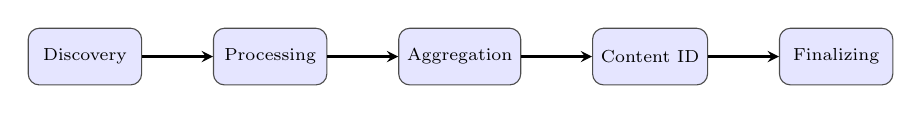
\begin{tikzpicture}[
    scale=0.9,
    transform shape,
    node distance=1.0cm,
    auto,
    phase/.style={rectangle, rounded corners, draw=black!70, fill=blue!10, minimum width=1.6cm, minimum height=0.8cm, align=center, font=\scriptsize},
    arrow/.style={->, >=stealth, thick}
]
    \node[phase] (discovery) {Discovery};
    \node[phase, right=of discovery] (processing) {Processing};
    \node[phase, right=of processing] (aggregation) {Aggregation};
    \node[phase, right=of aggregation] (content) {Content ID};
    \node[phase, right=of content] (finalizing) {Finalizing};

    \draw[arrow] (discovery) -- (processing);
    \draw[arrow] (processing) -- (aggregation);
    \draw[arrow] (aggregation) -- (content);
    \draw[arrow] (content) -- (finalizing);
\end{tikzpicture}
\caption{The five phases of the Spacedrive indexing pipeline. The ephemeral engine runs only Phase 1 for instant in-memory browsing, while the persistent engine executes all five phases.}
\label{fig:indexing_pipeline}
\end{figure}

\begin{itemize}[noitemsep, topsep=0pt]
 \item \textbf{Discovery Phase}: The engine performs a recursive traversal of a \texttt{Location}'s file system. It applies a set of predefined filter rules to ignore system and hidden files, caches, and development directories (e.g., \texttt{.git}, \texttt{node\_modules}). During traversal, the system captures filesystem metadata including inodes and modification timestamps for each entry. Discovered items are collected into batches for efficient processing.

 \item \textbf{Processing Phase}: Each batch of discovered entries is processed to create or update records in the database. This phase includes \textbf{change detection}, which uses the captured inode and modification timestamp data to identify new, modified, or moved files, ensuring that only necessary database updates are performed.

 \item \textbf{Aggregation Phase}: For directories, the engine performs a bottom-up traversal to calculate aggregate statistics, such as total size and file counts. This pre-calculation makes directory size lookups an O(1) operation.

 \item \textbf{Content Identification Phase}: For files, this phase generates a content hash (CAS ID---Content-Addressed Storage Identifier) for deduplication using BLAKE3. The system creates globally deterministic v5 UUIDs from content hashes, enabling offline duplicate detection across all devices without coordination. This phase also performs file type detection using a combination of extension matching and magic byte analysis through the FileTypeRegistry. For media files, the system leverages bundled FFmpeg libraries to extract rich metadata including duration, codec information, bitrate, resolution, and frame rate---all stored in dedicated media data tables for efficient querying.

 \item \textbf{Finalizing Phase}: This phase completes post-processing tasks including final directory aggregate updates and processor dispatch. In Deep Mode, this phase triggers thumbnail generation, OCR processing, and other analysis jobs defined by installed extensions. The phase marks the indexing operation as complete and updates the location's last-indexed timestamp.

\end{itemize}

After a file's content and type are identified in Phase 4, the Finalizing phase can dispatch specialized, asynchronous jobs for deeper analysis. These jobs are registered and defined by installed extensions, allowing for a modular approach to intelligence. For example, a Photos extension might queue an \texttt{ImageAnalysisJob} for images, while a developer extension might trigger a \texttt{CodeAnalysisJob} for source files. This ensures that deeper analysis is only performed when relevant to the user's workflow and installed extensions.

\paragraph{Checkpoint Architecture and Resumability}

The indexing engine's design enables robust resumability critical for mobile devices and large libraries where indexing can span hours and face multiple interruptions.

\textbf{Checkpoint Mechanism}: Jobs checkpoint automatically after each batch. State serialization uses MessagePack for compact binary encoding. Each checkpoint captures:

\begin{itemize}[noitemsep, topsep=0pt]
 \item Current phase identifier
 \item Batch cursor position
 \item Set of processed entry IDs
 \item Phase-specific state (e.g., discovered paths queue, aggregation stack)
\end{itemize}

\textbf{Resumability Flow}: When an indexing job is interrupted:

\begin{enumerate}[noitemsep, topsep=0pt]
 \item Job interrupted (crash, user cancellation, device offline, low battery)
 \item Current state persisted to \texttt{jobs.db} with last completed phase
 \item On restart: Load serialized state from database
 \item Jump to last completed phase, skip already-processed entries
 \item Continue from checkpoint cursor position
\end{enumerate}

This transforms hours-long indexing operations into resilient, interruptible workflows. A user can index a 500GB photo library over multiple days, pausing for battery conservation or device shutdown, with zero redundant work on resume.

\textbf{Ephemeral Mode}: The indexer's ephemeral mode creates in-memory \texttt{Entry} records for unindexed paths, enabling three critical use cases:

\begin{itemize}[noitemsep, topsep=0pt]
 \item \textbf{Exploratory Browsing}: Users can explore external drives or removable media before committing to permanent indexing, with full metadata capabilities (tagging, organizing) available immediately
 \item \textbf{Remote Filesystem Access}: When browsing a peer device, lightweight ephemeral entries stream in real-time without polluting the local database
 \item \textbf{Lazy Refresh Navigation}: During directory browsing, existing indexed data displays instantly while a background validation job updates changed entries
\end{itemize}

These in-memory ephemeral entries appear indistinguishable from persisted entries in the UI, creating a unified browsing experience across indexed and non-indexed data.

\paragraph{Memory Optimizations for Ephemeral Indexing}

To make ephemeral mode practical for browsing millions of files, Spacedrive employs specialized data structures that reduce memory overhead from ~250 bytes per entry (naive approach) to approximately 50 bytes per entry---a 5× reduction.

\textbf{NodeArena Slab Allocator}: Instead of storing entries in a \texttt{HashMap<PathBuf, Entry>} with 64-bit pointers, the system uses a contiguous memory slab indexed by 32-bit integers. This \texttt{NodeArena} allocates \texttt{FileNode} entries sequentially and maintains a free list for reusing deleted slots. The 32-bit node IDs reduce pointer overhead by 50\% while improving cache locality through sequential memory layout.

\textbf{NameCache String Interning}: Filesystem names repeat heavily---\texttt{index.js}, \texttt{.DS\_Store}, \texttt{package.json} appear thousands of times in typical projects. The \texttt{NameCache} stores each unique string once in an \texttt{Arc<str>} pool and references them by 32-bit IDs. For a Node.js project with 1,000 packages each containing \texttt{index.js}, string interning stores "index.js" once (8 bytes) plus 1,000 references (4 KB) instead of 1,000 copies (8 KB), achieving 50\% reduction. Common names like \texttt{.git}, \texttt{README.md}, and system files deduplicate heavily across directory trees.

\textbf{NameRegistry for Fast Lookups}: A \texttt{BTreeMap<NameId, Vec<NodeId>} enables O(log n) "find by name" queries without full-text indexing. This allows instant lookups like "find all README.md files" by indexing on interned name IDs rather than string comparisons.

These optimizations enable browsing hundreds of thousands of files in ephemeral mode with under 50 MB of RAM, making Spacedrive viable as a daily-driver file manager for exploring external drives and network shares without database commits.

\subsubsection{Flexible Indexing Scopes and Persistence}
\label{sec:indexing-scopes}
A key innovation of the Spacedrive indexer is its ability to adapt to different use cases through two orthogonal dimensions: \textbf{scope} and \textbf{persistence mode}.

\textbf{Indexing Scope}: The indexer can perform either a full recursive scan of a directory tree or a shallow, single-level scan of immediate contents. The shallow mode is integral to Spacedrive's responsive UI navigation through a "lazy refresh" mechanism—when browsing directories, the system instantly presents existing indexed data while concurrently spawning a non-blocking validation job to ensure accuracy without sacrificing interactivity.

\textbf{Persistence Mode}: For managed \texttt{Locations}, indexing results are persisted to the Library's database. However, the indexer also supports an \textbf{ephemeral, in-memory mode}. First, users can browse external or temporary paths without polluting the main index; the system generates temporary \texttt{Entry} records on the fly, streaming them to the UI for responsive exploration. Second, this extends to \textbf{remote filesystems}—when a user browses a path on a paired device, Spacedrive initiates an ephemeral indexing job on the target device, streaming lightweight \texttt{Entry} records back in real time. These ephemeral entries, whether local or remote, are presented "inline" with persisted entries, creating a unified view of the distributed filesystem.

This flexibility is managed through a unified \texttt{IndexerJobConfig}, enabling fine-grained control from background library maintenance to real-time UI interactions.

\subsubsection{Locations and Real-Time Monitoring}

A Spacedrive Library is composed of one or more \textbf{Locations}---managed directories that act as the entry points to a user's physical file systems. The \textbf{Location Watcher} service provides a cross-platform, real-time monitoring system that keeps the Spacedrive index synchronized with the underlying file system.

\textbf{The Location as a Managed Entity}

When a user adds a directory to a Spacedrive Library, it becomes a \texttt{Location}, a managed entity with its own configuration and lifecycle. Each Location provides granular control over how different parts of the user's data space are handled. Each \texttt{Location} has a specific \textbf{Index Mode} (\texttt{Shallow}, \texttt{Content}, or \texttt{Deep}), enabling users to apply different levels of analysis to different types of content (e.g., deep analysis for a photo library, shallow for a downloads folder).

\textbf{The Location Watcher Service}

The watcher service is the core of Spacedrive's real-time capabilities, providing an efficient file system monitoring solution.

\textbf{Platform-Specific Optimizations}

A key strength of the watcher is its use of platform-native APIs for optimal performance and reliability. This is a non-trivial engineering challenge, as each OS has unique behaviors.

\begin{itemize}[noitemsep, topsep=0pt]
 \item \textbf{macOS (\texttt{FSEvents})}: The system correctly handles the ambiguous rename and move events from \texttt{FSEvents} by tracking file inodes to reliably link old and new paths.

 \item \textbf{Linux (\texttt{inotify})}: The watcher leverages the efficiency of \texttt{inotify} for direct, recursive directory watching and uses cookie-based event correlation to reliably detect move operations.

 \item \textbf{Windows (\texttt{ReadDirectoryChangesW})}: The implementation is designed to handle Windows-specific filesystem quirks, such as delayed file deletions caused by antivirus software or file locking. It does this by maintaining a "pending deletion" state to verify that a file is truly gone before emitting a deletion event.
\end{itemize}

\textbf{Event Processing Pipeline}

The watcher service is more than a simple event forwarder. It includes a processing pipeline:

\begin{itemize}[noitemsep, topsep=0pt]
 \item \textbf{Noise Filtering via IndexerRuler}: The watcher applies the same configurable \textbf{indexer rules engine} used during initial indexing through the \texttt{IndexerRuler} component. This unified filtering system provides toggleable system rules including \texttt{NO\_HIDDEN} (skip dotfiles like \texttt{.git}, \texttt{.DS\_Store}), \texttt{NO\_DEV\_DIRS} (skip \texttt{node\_modules}, \texttt{target}, \texttt{dist}), \texttt{NO\_SYSTEM} (skip OS folders like \texttt{System32}, \texttt{/proc}), and \texttt{NO\_TEMP} (skip temporary files). When indexing inside Git repositories, the ruler automatically loads and applies \texttt{.gitignore} patterns, preventing build artifacts and local configuration from polluting the index. Rules are evaluated at the discovery edge---rejected files never enter the processing pipeline, providing 6-8× speedup on typical development directories by avoiding expensive database operations for thousands of dependency files.

 \item \textbf{Event Debouncing}: To prevent "event storms" during bulk operations (e.g., unzipping an archive), the system debounces file system events, consolidating rapid-fire changes into single, actionable events.

 \item \textbf{Responder Pipeline}: Processed events are dispatched to the \textbf{indexer responder}, which translates raw filesystem events into database operations. The responder resolves entry identities, updates metadata, triggers content processors (thumbnails, OCR, content hashing), and emits resource events that notify the sync service to propagate changes to other devices.
\end{itemize}

This real-time monitoring system helps Spacedrive maintain an up-to-date view of a user's files.

\subsubsection{Offline Recovery and Stale Detection}
\label{sec:offline-recovery}

While the Location Watcher provides real-time monitoring during normal operation, a critical challenge arises when Spacedrive itself is offline---whether due to system shutdown, crashes, or disconnected storage volumes. When the system returns online, it must efficiently detect and reconcile any filesystem changes that occurred during its absence.

\textbf{Design for Offline Window Tracking}

The system architecture includes support for tracking watcher uptime and persisting last-shutdown timestamps per location. Upon startup, the planned behavior is to calculate the "offline window"---the period between the last shutdown and current time---defining the temporal scope for potential undetected changes. By comparing this offline period against filesystem modification times, the system can efficiently identify which portions of the filesystem require validation. Note that while the change detection infrastructure (ChangeDetector) and verification system (IndexVerifyAction) are implemented, \textit{automatic startup stale detection is not yet fully deployed}. Currently, users can manually trigger verification via CLI commands when needed.

\textbf{Stale Detection Algorithm}

Rather than performing expensive full filesystem scans after every offline period, Spacedrive leverages a key property of modern filesystems: modification time propagation. On most operating systems (Windows NTFS, macOS APFS, and Linux ext4/btrfs), changes to files within nested directories update the modification timestamps of parent directories up the tree.

The stale detection algorithm operates as follows:
\begin{enumerate}[noitemsep, topsep=0pt]
\item Walk the directory tree starting from each Location root
\item Compare directory modification times against the offline window
\item If a directory's modification time falls within the offline window, mark it for deep scanning
\item Recursively scan only marked directories and their contents
\item Update the index with discovered changes while preserving unchanged portions
\end{enumerate}

This approach substantially reduces re-indexing overhead. For example, in a Location with 100,000 files across 10,000 directories where only 50 files changed during offline time, the system might only need to deeply scan 200–300 directories rather than the entire tree.

\textbf{Graceful Degradation for Unsupported Filesystems}

For filesystems that don't reliably propagate modification times (such as certain network filesystems or FAT32), Spacedrive detects this limitation and falls back to an ephemeral deep indexing strategy. This approach leverages the existing multi-phase indexing pipeline but constrains execution to only the Discovery phase---rapidly traversing the filesystem to create lightweight Entry records without performing expensive content analysis. By comparing these ephemeral entries against the persisted database state, the system can efficiently identify additions, deletions, and modifications based on file metadata. Only the detected changes are then queued for full processing through the remaining indexing phases (content identification, media analysis, etc.). The system maintains filesystem capability profiles to automatically select the optimal detection strategy per Location.

This hybrid approach ensures Spacedrive maintains its performance advantages while guaranteeing index integrity, addressing a fundamental limitation of purely real-time monitoring systems.

\subsubsection{Index Verification and Integrity Checking}

To provide diagnostic capabilities and ensure index correctness, Spacedrive implements an \texttt{IndexVerifyAction} that performs on-demand integrity checks. This system runs a fresh ephemeral scan of a location and compares the in-memory results against the persistent database, identifying discrepancies without modifying any data.

The verification process detects three categories of integrity issues: \textbf{MissingFromIndex} (files exist on disk but not in database, indicating missed create events or indexing gaps), \textbf{StaleInIndex} (entries in database but files missing from filesystem, indicating missed delete events), and \textbf{MetadataMismatch} (size, modification time, or inode differences between database and filesystem, indicating missed modify events or filesystem corruption). Each issue includes the affected path, entry ID, and specific mismatch details.

The verification system generates detailed \texttt{IntegrityReport} outputs with per-file diagnostics and summary statistics, accessible via CLI commands or the UI. This is particularly valuable after extended offline periods, when debugging watcher issues, or before major library migrations. The ephemeral comparison approach---indexing into memory rather than database---ensures verification runs quickly (typically under 30 seconds for 100K files) and never corrupts the existing index. Users can trigger verification manually via \texttt{spacedrive verify <path>} or schedule periodic background checks for critical locations.

\subsubsection{Extending the Indexer for Remote Volumes}
\label{sec:remote-volumes}

Spacedrive's indexing pipeline extends naturally to remote volumes (e.g., cloud services like S3 or protocols like FTP) through integration with OpenDAL~\cite{opendal-2025}, a Rust-native library providing unified, asynchronous access to diverse storage backends. This allows treating remote storage as standard Locations without data duplication, leveraging ranged reads for efficiency and provider metadata for optimized hashing.

\textbf{Key Adaptations:}
\begin{itemize}[noitemsep, topsep=0pt]
\item \textbf{Discovery Phase}: Use OpenDAL's \texttt{Lister} for streaming directory traversal, avoiding full loads for large remotes (e.g., petabyte S3 buckets).
\item \textbf{Content Identification}: Prioritize provider-computed hashes where available (e.g., S3 ETag as MD5 for small files~\cite{aws-s3-etag-2025}; GCS MD5). Fallback to client-side adaptive hashing via ranged reads to sample chunks without full downloads.
\item \textbf{Resilience}: Wrap operations in retries with exponential backoff to handle rate limits (e.g., S3's 3,500 requests/sec) and transient errors.
\item \textbf{Metadata-Only Mode}: Initial indexing fetches only stats (size, mod time) for quick Entry creation; defer content analysis to on-demand jobs.
\end{itemize}

This design minimizes bandwidth and costs: hashing a 10GB file uses only ~64KB of ranged data (8KB header + 4×10KB samples + 8KB footer) instead of full transfer. The implementation builds scheme-specific OpenDAL operators (for S3, FTP, etc.) from location configuration, retrieving credentials from the secure vault. Remote hashing applies the same adaptive BLAKE3 strategy as local files, using ranged reads for efficient sampling without downloading entire files. Recent OpenDAL enhancements (v0.49, 2025) improve concurrent listing and metadata handling~\cite{opendal-changelog-2025}.

\subsubsection{High-Performance Hierarchical Indexing}
To overcome the scaling limitations of traditional path-based queries, Spacedrive's index uses a \textbf{Closure Table} for all hierarchical data. This database pattern pre-calculates and stores all ancestor-descendant relationships in an \texttt{EntryClosure} table, transforming slow string comparisons into highly efficient, indexed integer joins.

When a new entry is created, its \texttt{parent\_id} is used to transactionally populate the \texttt{entry\_closure} table with all its ancestor relationships in a single, atomic operation. This keeps the hierarchy consistent.

A critical component of this system is the indexer's resilient change detection. To ensure data integrity, especially for offline changes, the indexer uses \textbf{inode tracking} to reliably differentiate between a file move and a delete/add operation. When a file is moved within the same volume, its inode remains constant. The indexer leverages this to identify the operation as a move, triggering a safe, transactional update of the entry's path and its position in the closure table, rather than performing a destructive and incorrect delete-and-re-add. This preserves all user metadata and ensures the integrity of the hierarchical index.

% --- SECTION 4.4: THE TRANSACTIONAL ACTION SYSTEM ---
\subsection{The Transactional Action System}
\label{sec:action-system}

\begin{keytakeaways}
\begin{itemize}[noitemsep, topsep=0pt]
\item \textbf{New Paradigm}: Preview any operation before execution - see exactly what will happen
\item \textbf{Durable Execution}: Operations become durable jobs that continue across device disconnections
\item \textbf{Centralized Control}: All operations flow through type-safe action system with full audit logging
\end{itemize}
\end{keytakeaways}

Traditional file management executes operations immediately without preview. Spacedrive's \textbf{Transactional Action System with Pre-visualization} treats operations as transactions that can be previewed.

This system allows any file system operation to be simulated in a "dry run" mode before execution. Powered by the VDFS library index, this simulation can pre-visualize the outcome of an action---including space savings, data deduplication, and the final state of all affected locations---without touching a single file.

\subsubsection{The Action Lifecycle: Preview, Commit, Verify}

Every action in Spacedrive follows a transactional lifecycle:

\textbf{Intent \& Preview}: The user expresses an intent (e.g., "move photos from my phone to my NAS"). Spacedrive uses its index to generate a preview of the outcome. The system can accurately forecast the end state because it has a complete metadata map of all user data.

\textbf{Commit}: Once the user approves the preview, the action is committed to the Durable Job System. It becomes a resilient, resumable job that continues to execute when devices are online, even if network connectivity is intermittent.

\textbf{Execution \& Verification}: The job is executed by the appropriate device agents when they come online. The system works to complete the job, verifying each step against the initial plan. This durability helps ensure that user intent is fulfilled without data loss or corruption.

\begin{figure}[ht!]
\centering
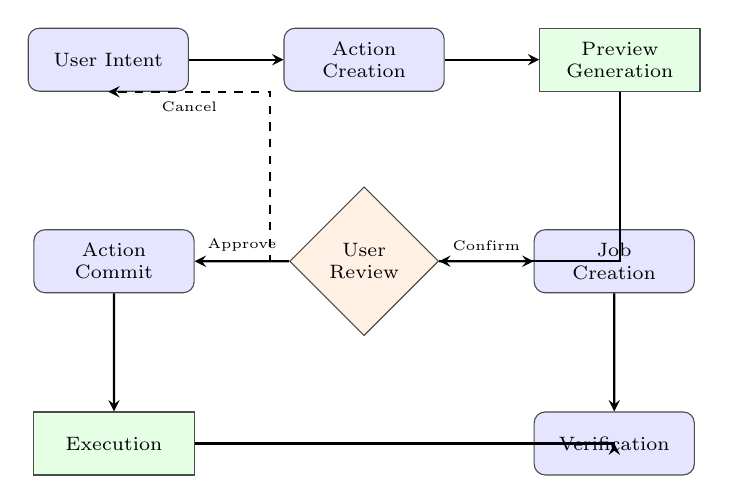
\begin{tikzpicture}[
    scale=0.8,
    node distance=1.5cm and 1.2cm,
    auto,
    state/.style={rectangle, rounded corners, draw=black!70, fill=blue!10, text width=1.8cm, minimum height=0.8cm, align=center, font=\scriptsize},
    decision/.style={diamond, draw=black!70, fill=orange!10, text width=1.3cm, minimum height=0.8cm, align=center, font=\scriptsize, inner sep=1pt},
    process/.style={rectangle, draw=black!70, fill=green!10, text width=1.8cm, minimum height=0.8cm, align=center, font=\scriptsize},
    arrow/.style={->, >=stealth, thick},
    label/.style={font=\tiny, align=center}
]
    % Top row
    \node[state] (intent) {User Intent};
    \node[state, right=of intent] (action) {Action\\Creation};
    \node[process, right=of action] (preview) {Preview\\Generation};

    % Bottom row
    \node[decision, below=1.2cm of action] (review) {User\\Review};
    \node[state, left=of review] (commit) {Action\\Commit};
    \node[state, right=of review] (job) {Job\\Creation};

    % Execution nodes
    \node[process, below=of commit] (execute) {Execution};
    \node[state, below=of job] (verify) {Verification};

    % Arrows
    \draw[arrow] (intent) -- (action);
    \draw[arrow] (action) -- (preview);
    \draw[arrow] (preview) |- (review);
    \draw[arrow] (review) -- node[label, above] {\tiny Approve} (commit);
    \draw[arrow] (review) -- node[label, above] {\tiny Confirm} (job);
    \draw[arrow] (commit) -- (execute);
    \draw[arrow] (job) -- (verify);
    \draw[arrow] (execute) -| (verify);

    % Cancel path
    \draw[arrow, dashed] (review.west) -- ++(-0.3,0) |- node[label, near end] {\tiny Cancel} (intent.south);
\end{tikzpicture}
\caption{The Action Lifecycle: From user intent through preview, approval, and execution}
\label{fig:action-lifecycle}
\end{figure}

\begin{figure}[ht!]
\centering
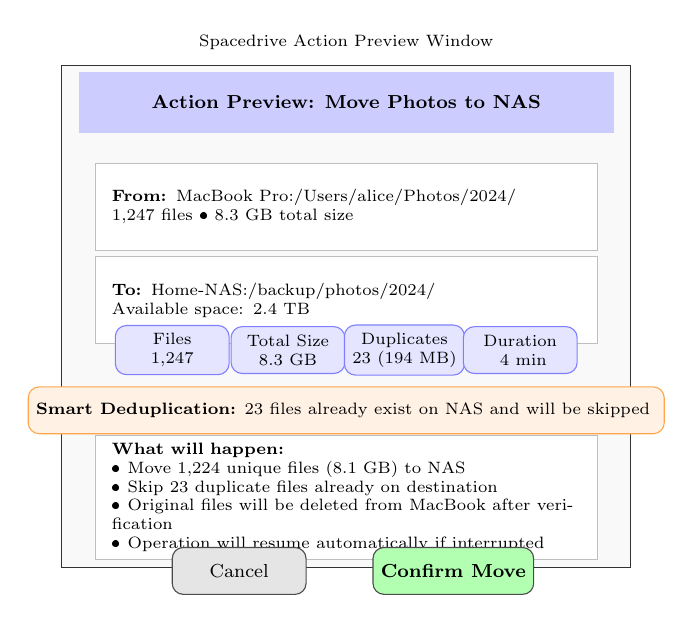
\begin{tikzpicture}[
    scale=0.85,
    transform shape,
    % UI Frame
    uiframe/.style={rectangle, draw=black!80, fill=gray!5, minimum width=8.5cm, minimum height=7.5cm},
    % UI Elements
    header/.style={rectangle, fill=blue!20, minimum width=8cm, minimum height=0.9cm, align=center, font=\footnotesize\bfseries},
    section/.style={rectangle, draw=gray!50, fill=white, minimum width=7.5cm, minimum height=1.3cm, align=left, font=\scriptsize},
    button/.style={rectangle, rounded corners, draw=black!70, minimum width=2cm, minimum height=0.7cm, align=center, font=\footnotesize},
    cancelbutton/.style={button, fill=gray!20},
    confirmbutton/.style={button, fill=green!30},
    stat/.style={rectangle, rounded corners, draw=blue!50, fill=blue!10, minimum width=1.7cm, minimum height=0.7cm, align=center, font=\scriptsize},
    warningbox/.style={rectangle, rounded corners, draw=orange!70, fill=orange!10, minimum width=7.5cm, minimum height=0.7cm, align=center, font=\scriptsize}
]
    % Main Frame
    \node[uiframe] (frame) {};

    % Header
    \node[header] at (0, 3.2) {Action Preview: Move Photos to NAS};

    % Source Section
    \node[section, anchor=north, text width=7cm] at (0, 2.3) (source) {
        \textbf{From:} MacBook Pro:/Users/alice/Photos/2024/\\
        \scriptsize 1,247 files • 8.3 GB total size
    };

    % Destination Section
    \node[section, anchor=north, text width=7cm] at (0, 0.9) (dest) {
        \textbf{To:} Home-NAS:/backup/photos/2024/\\
        \scriptsize Available space: 2.4 TB
    };

    % Statistics Row
    \node[stat] at (-2.6, -0.5) {Files\\1,247};
    \node[stat] at (-0.87, -0.5) {Total Size\\8.3 GB};
    \node[stat] at (0.87, -0.5) {Duplicates\\23 (194 MB)};
    \node[stat] at (2.6, -0.5) {Duration\\~4 min};

    % Deduplication Notice
    \node[warningbox] at (0, -1.4) {
        \textbf{Smart Deduplication:} 23 files already exist on NAS and will be skipped
    };

    % Preview Details
    \node[section, minimum height=1.7cm, text width=7cm] at (0, -2.7) {
        \textbf{What will happen:}\\
        \scriptsize
        • Move 1,224 unique files (8.1 GB) to NAS\\
        • Skip 23 duplicate files already on destination\\
        • Original files will be deleted from MacBook after verification\\
        • Operation will resume automatically if interrupted
    };

    % Buttons
    \node[cancelbutton] at (-1.6, -3.8) {Cancel};
    \node[confirmbutton] at (1.6, -3.8) {\textbf{Confirm Move}};

    % Title
    \node[font=\scriptsize, above=0.1cm of frame.north] {Spacedrive Action Preview Window};
\end{tikzpicture}
\caption{Action Preview UI Mockup: Users see exactly what will happen before any files are modified, including deduplication savings and potential issues.}
\label{fig:action-preview-ui}
\end{figure}

\paragraph{Accessibility Integration}
The UI supports screen readers for natural language commands and high-contrast modes for previews, ensuring inclusive AI access~\cite{wcag-2021}.

\subsubsection{The Simulation Engine}

The Spacedrive index serves as the basis for a simulation engine that provides accurate operation previews through complete knowledge of the VDFS state.

\paragraph{Index-Based Simulation Architecture}

The simulation engine's power derives from having complete metadata for every file without filesystem access:

\begin{itemize}[noitemsep, topsep=0pt]
 \item \textbf{Zero I/O Preview}: All predictions via SQL queries against the VDFS index—no filesystem reads during preview generation
 \item \textbf{Complete Knowledge}: Every file's size, content hash, location, permissions, and relationships are instantly available
 \item \textbf{Deduplication Awareness}: Content Identity table enables instant duplicate detection across all devices
 \item \textbf{Hierarchical Operations}: Closure table enables O(1) queries for directory subtrees, avoiding recursive scans
\end{itemize}

This architecture transforms operation planning from a slow, I/O-bound process into a fast, in-memory query execution.

\paragraph{Content-Aware Path Resolution}

For operations using \texttt{SdPath::Content} addressing, the simulation engine performs optimal path resolution through a cost function evaluation:

\begin{enumerate}[noitemsep, topsep=0pt]
 \item \textbf{Content Lookup}: Query Content Identity table for all file instances across all devices
 \item \textbf{Candidate Evaluation}: Score each instance using a cost function:
   \begin{itemize}[noitemsep]
     \item \textbf{Locality}: Local device copies = 0 cost (instant access)
     \item \textbf{Network Proximity}: Iroh provides real-time latency/bandwidth estimates per peer
     \item \textbf{Storage Tier}: PhysicalClass prioritizes SSD over HDD for source files
     \item \textbf{Device Availability}: Filter for currently online devices only
   \end{itemize}
 \item \textbf{Path Selection}: Select lowest-cost valid path; simulation proceeds with this resolved path
\end{enumerate}

This enables accurate time estimation even when the optimal source device differs from the user's assumption.

\textbf{Operational Conflict Detection}

The closure table also significantly accelerates the preview generation itself. When simulating a move or copy of a large directory, the system can determine the entire scope of the operation (all descendant files and folders) with a single, efficient query, rather than a slow recursive path scan. The simulation engine identifies operational conflicts that would cause traditional file operations to fail:
\begin{itemize}[noitemsep, topsep=0pt]
\item \textbf{Storage Constraints}: Calculates exact space requirements and verifies availability on target devices
\item \textbf{Permission Violations}: Detects write-protected locations or access-restricted files before attempting operations
\item \textbf{Path Conflicts}: Identifies naming collisions and circular reference issues in complex move operations
\item \textbf{Resource Limitations}: Estimates memory and bandwidth requirements against device capabilities
\end{itemize}

The simulation engine catches operational conflicts during planning, while Library Sync's per-model resolution handles the rare synchronization conflicts from concurrent modifications (Section~\ref{sec:library-sync}). This dual approach improves reliability in distributed file management.

This is particularly powerful when combined with Native Storage Tiering (Section~\ref{sec:volume-foundation}). If a user attempts an operation on a Location they have marked with a \texttt{Hot} logical class, but it resides on a Volume physically classified as \texttt{Cold}, the simulation engine generates a clear warning in the preview: "\textbf{Warning:} This operation targets a 'hot' location on a slow archive drive. Estimated completion time may be longer than expected."

\paragraph{Time Estimation}
The Simulation Engine combines multiple data sources to provide accurate operation time estimates:

\begin{itemize}
    \item \textbf{Volume Performance Metrics}: Real-time read/write speeds from continuous monitoring
    \item \textbf{Network Conditions}: Current bandwidth and latency from Iroh's measurements
    \item \textbf{Historical Data}: Previous operations on similar files and paths
    \item \textbf{Operation Complexity}: Number of files, total size, and fragmentation
    \item \textbf{Storage Type Awareness}: Different strategies for local vs cloud storage
\end{itemize}

For example, when copying 10GB across devices, the estimation considers:
\begin{itemize}
    \item Source volume read speed: 250 MB/s (measured)
    \item Network throughput: 45 MB/s (current P2P bandwidth)
    \item Destination write speed: 180 MB/s (measured)
    \item Bottleneck: Network at 45 MB/s
    \item Estimated time: 3 minutes 45 seconds (with 10\% buffer)
\end{itemize}

For cloud operations, additional factors apply:
\begin{itemize}
    \item API rate limits (e.g., 1000 requests/second for S3)
    \item Chunk size optimization (balancing throughput vs memory)
    \item Parallel stream count (typically 4-8 for cloud providers)
    \item Resume capability for long-running transfers
\end{itemize}

This transparency helps users make informed decisions about when and how to execute operations, especially for large-scale cloud migrations.

\subsubsection{Centralized Operation Control}

Rather than allowing direct operation dispatch throughout the codebase, Spacedrive routes all user actions through a centralized \textbf{Action System} that provides consistent validation, execution, and logging:

The Action System employs a centralized enumeration that captures every possible user operation, distinguishing between global actions (system-level operations like library creation) and library-scoped actions (operations within a specific Library context). This design provides clear authorization boundaries and enables complete tracking of all user-initiated operations.

\subsubsection{Type-Safe Action Construction}

The system employs a \textbf{builder pattern} for type-safe action construction that integrates with CLI and API inputs:

\begin{lstlisting}[language=Rust, caption={Type-safe action construction with builder pattern}]
// Builder pattern ensures valid action construction
let action = FileCopyAction::builder()
    .source_paths(vec!["/docs/report.pdf", "/docs/data.csv"])
    .target_path("/backup/2024/")
    .mode(TransferMode::Move)  // Move instead of copy
    .verify_checksum(true)      // Ensure integrity
    .preserve_timestamps(true)   // Keep original dates
    .on_conflict(ConflictStrategy::Skip)
    .build()?;  // Returns error if invalid combination

// Actions are serializable for durability
let job = Job::from_action(action);
queue.push(job).await?;
\end{lstlisting}

This builder approach provides \textbf{compile-time validation} of action parameters, preventing invalid operations from reaching the execution layer while maintaining ergonomic APIs for both programmatic and command-line usage.

\subsubsection{Complete Audit Logging}

Every library-scoped action automatically receives full audit logging through the database layer:

\begin{table}[h]
\footnotesize
\centering
\begin{tabular}{@{}ll@{}}
\toprule
\textbf{Audit Field} & \textbf{Information Captured} \\
\midrule
Action Type & Operation performed (e.g., "file.copy") \\
Device & Initiating device identifier \\
Resources & Files/folders/locations affected \\
Status & Previewed → Committed → Complete \\
Job Link & Background job reference \\
Timing & Start/end times, duration \\
Errors & Failure details if applicable \\
Results & Outcome and metrics \\
\bottomrule
\end{tabular}
\caption{Detailed audit trail fields}
\label{tab:audit-fields}
\end{table}

The \textbf{ActionManager} automatically creates audit entries for both preview and execution phases, tracking the complete action lifecycle from initial intent through final completion.

\subsubsection{Dynamic Handler Registry}

The Action System employs a dynamic registry pattern using Rust's \textbf{inventory} crate for automatic handler discovery:

\textbf{Extensible Action Handler System}

Spacedrive's Action System uses a self-registering architecture that automatically discovers available operations:

\begin{itemize}[noitemsep, topsep=0pt]
 \item \textbf{Automatic Discovery}: New operations register themselves when added to the codebase
 \item \textbf{No Central Maintenance}: Adding new file operations requires no manual registry updates
 \item \textbf{Type Safety}: Each operation handler is validated at compile time
 \item \textbf{Consistent Interface}: All operations (file copy, location management, etc.) follow the same patterns
\end{itemize}

This enables easy extension of Spacedrive's capabilities while maintaining system reliability and consistent user experience across all operations.

\subsubsection{Foundation for Advanced Capabilities}

The Action System's centralized architecture enables advanced features that would be difficult to implement across a distributed codebase:

\textbf{\plannedSection{Enterprise-Grade RBAC Foundation}}

The centralized Action System is architected as the foundation for granular Role-Based Access Control (RBAC), essential for team collaboration and enterprise deployment:

\begin{itemize}[noitemsep, topsep=0pt]
 \item \textbf{Role Definitions}: Standard roles like "Viewer" (read-only), "Contributor" (read/write), "Manager" (full control), and custom roles tailored to organizational needs
 \item \textbf{Granular Permissions}: Action-level control enabling scenarios like "can upload but not delete" or "can tag but not move files"
 \item \textbf{Location-Based Access}: Restrict access to specific Locations or paths (e.g., "Finance team accesses /financial-data, Creative team accesses /assets")
 \item \textbf{Inheritance and Groups}: Permission inheritance through organizational groups with override capabilities
 \item \textbf{Temporal Controls}: Time-based access for contractors or temporary project members
 \item \textbf{Audit Trail Integration}: Every permission check logged with full context for compliance and security reviews
\end{itemize}

\textbf{\plannedSection{Undo Capabilities}}

The detailed audit trail provides the foundation for reliable operation reversal:

\begin{itemize}[noitemsep, topsep=0pt]
 \item \textbf{Safe Undo Logic}: System understands how to safely reverse each operation type
 \item \textbf{Dependency Tracking}: Prevents undoing operations that other actions depend on
 \item \textbf{Selective Reversal}: Undo specific parts of complex operations (e.g., "undo copying just these 3 files")
 \item \textbf{Cross-Device Coordination}: Undo operations that span multiple devices with proper cleanup
\end{itemize}

\subsubsection{Remote Action Dispatch}

A key benefit of combining the Action System with the \texttt{SdPath} universal addressing scheme is the ability to dispatch actions where the execution occurs transparently on a remote device. For example, a \texttt{FileCopyAction} can specify a source \texttt{SdPath} on Device A and a destination \texttt{SdPath} on Device B. When this action is committed, the Job System routes the work to the appropriate device. It creates a sender job on Device A and a corresponding receiver job on Device B, which coordinate the transfer over the secure P2P network. This architecture makes complex cross-device workflows trivial to express and execute, as the underlying network communication and state management are handled automatically by the core engine. All remote operations are still subject to the same validation, preview, and audit logging as local actions, ensuring a consistent security model across the entire VDFS.

\subsubsection{Handling File Ingestion and Uploads}
\label{sec:ingestion-workflow}
While much of Spacedrive's power comes from indexing existing files, a critical function is the ingestion of new files from external sources, such as a web interface or a drag-and-drop operation into the application. This process is managed through a specialized \textbf{Ingestion Workflow}, built upon the Transactional Action System.

At the heart of this workflow is the concept of a user-configurable \textbf{Ingest Location}, colloquially known as an "Inbox" or "quarantine zone." This is a designated default directory on a preferred, often always-online, device (such as a home server or a Cloud Core instance). When a user uploads a file without specifying an explicit destination:

\begin{enumerate}[noitemsep, topsep=0pt]
    \item A \texttt{FileIngestAction} is created. The source is the uploaded data stream, and the destination defaults to the primary Ingest Location.
    \item The Action System routes this job to the destination device, which handles the secure file transfer via the Iroh protocol.
    \item Upon successful transfer, the file is written to the Ingest Location, and a new \texttt{Entry} is created in the VDFS index.
\end{enumerate}

This architecture ensures that new files are added to the user's data space in a transactional, reliable manner. Once the file becomes a managed \texttt{Entry}, it is immediately available for the AI layer to analyze and organize, as detailed in Section~\ref{sec:ai-native-ingestion}.

% --- SECTION 4.5: LIBRARY SYNC & NETWORKING ---
\subsection{Library Sync and Networking}
\label{sec:sync-networking}

Spacedrive's distributed architecture requires synchronization and networking capable of maintaining consistency across devices while preserving local-first semantics. This section presents the approach to synchronization through domain separation and the Iroh-powered networking infrastructure~\cite{iroh_networking} that enables peer-to-peer communication.

\subsubsection{Library Sync via Domain Separation}
\label{sec:library-sync}

Traditional distributed consensus algorithms struggle with the mixed requirements of personal data management. Spacedrive's Library Sync architecture sidesteps this complexity through a leaderless, peer-to-peer hybrid model that aligns synchronization strategy with data ownership. The key insight is that personal file management exhibits a natural ownership hierarchy: each device has exclusive authority over its local filesystem, while user-generated metadata (tags, collections) represents truly shared state that any device may modify.

This domain separation eliminates central coordinators, single points of failure, and the need for leader election. Data falls into two categories with tailored replication strategies.

\paragraph{Device-Authoritative Data}

Each device maintains authoritative control over its own filesystem index. Ownership flows through volumes: each device owns its attached volumes, and locations and entries inherit ownership from their volume. This indirection enables portable storage---when an external drive moves between machines, a single volume update transfers ownership of all associated data instantly. Since no other device can modify another's local filesystem, write conflicts for this data class are impossible by construction. Synchronization employs a per-resource watermark system that enables efficient incremental sync.

Rather than tracking sync progress globally, the system maintains independent watermarks for each resource type (locations, entries, volumes). This granular approach enables targeted recovery: if entry synchronization falls behind, only entries require re-syncing while location and volume sync remain unaffected. Each watermark advances only when data is actually received---a critical invariant that prevents data loss when network requests return empty results.

When devices reconnect after an offline period, incremental catch-up requests only records newer than the stored watermark. The response uses cursor-based pagination with a \texttt{timestamp|uuid} format to handle large result sets and ensure no records are skipped even when timestamps collide. If a watermark exceeds a configurable age threshold (default 25 days), the system forces a full sync to ensure consistency, as tombstones for deletions may have been pruned beyond that point.

\paragraph{Shared Data}

User-generated metadata such as tags and collections is not owned by any single device and can be modified concurrently. This domain uses a lightweight, log-based approach where each device maintains a small per-device log (\texttt{sync.db}) of changes to shared resources. Each entry carries a Hybrid Logical Clock (HLC) timestamp---a distributed timestamp combining physical time with a logical counter that provides total ordering across all devices without clock synchronization.

The HLC structure encodes timestamp, counter, and device identifier:
\begin{equation}
\text{HLC} = (\text{timestamp}_{64}, \text{counter}_{64}, \text{device\_id}_{128})
\end{equation}

Comparison proceeds lexicographically: first by timestamp, then counter, then device ID. This guarantees a total ordering over all events in the system, enabling deterministic conflict resolution regardless of the order in which devices receive updates.

Conflict resolution is per-model. Tag assignments use implicit union merge---when two devices tag the same file with different tags, both assignments sync as separate records and the file ends up with all tags. Scalar values such as favorites use last-writer-wins based on HLC ordering. These logs are aggressively pruned once all peers acknowledge receipt, typically maintaining fewer than 1,000 entries even with active multi-device usage.

\paragraph{Explicit File Transfer}

Unlike automatic synchronization, file movements and copying in Spacedrive are explicit user commands. When a user requests ``copy my photos to the backup drive,'' this creates a deliberate operation with clear source and destination specifications, predictable error handling with retry logic, and progress tracking. This separation eliminates the complexity of implicit file content synchronization, treating transfers as user-initiated operations with well-defined semantics.

The leaderless architecture provides several practical advantages. Any device can make changes without waiting for a coordinator. Devices queue changes locally and sync when connectivity returns, enabling true offline-first operation without read-only restrictions. No single point of failure exists---any peer can provide synchronization state to new devices. The absence of leader election, heartbeat mechanisms, and failover logic results in approximately 800 fewer lines of coordination code compared to leader-based alternatives.

\subsubsection{Iroh-Powered Network Infrastructure}

Spacedrive's networking architecture consolidates sync, file transfer, and device discovery into a unified layer powered by Iroh. Rather than managing separate networking stacks for each protocol, all communication flows through a single QUIC endpoint per device.

\paragraph{Protocol Multiplexing}

Application-Layer Protocol Negotiation (ALPN) enables multiple Spacedrive protocols to coexist on a single QUIC connection. One connection per device pair handles pairing, sync, file transfer, and messaging, with each protocol identified by its ALPN string (e.g., \texttt{spacedrive/sync/1}). Protocols become streams rather than separate connections, sharing congestion control and eliminating coordination overhead. This consolidation reduces connection establishment time to under 2 seconds (from 3--5 seconds with separate connections) and eliminates approximately 60\% of networking coordination code.

To prevent race conditions inherent in peer-to-peer networks, Spacedrive employs deterministic connection roles: only the device with the lexicographically lower NodeId initiates outbound connections. This eliminates simultaneous connection attempts and simplifies the connection state machine, as each device knows its role (initiator or responder) deterministically and consistently across reconnection attempts.

\paragraph{Pairing and Security}

Initial device pairing employs a challenge-response protocol built on BIP39 mnemonic codes---12-word phrases derived from 256-bit secrets that provide human-readable verification. The four-message handshake prevents replay attacks, while Ed25519 signatures provide cryptographic authentication against man-in-the-middle attacks. Visual device fingerprints offer an additional verification layer during initial pairing.

The underlying QUIC transport provides ChaCha20-Poly1305 encryption, stream multiplexing for concurrent operations, BBR congestion control, and zero round-trip connection resumption. All traffic is encrypted end-to-end regardless of the network path.

\paragraph{Network Discovery and Relay}

Devices discover each other through multiple channels simultaneously: local network mDNS broadcasting, DNS-based discovery for known devices, and relay server coordination for NAT traversal. When direct connection is not possible due to firewalls or symmetric NAT, the system routes through relay servers while maintaining end-to-end encryption---relays see only encrypted traffic and cannot inspect content.

While Spacedrive provides public relay servers, the architecture supports self-hosted deployments for organizations requiring data sovereignty or operating air-gapped networks. The relay service deploys as a single binary with minimal configuration, enabling geographic distribution near users for optimal latency. This flexibility accommodates enterprises with data residency requirements and organizations building private overlay networks.

\paragraph{Network Topologies}
The Iroh-based networking supports multiple deployment topologies:

\begin{figure}[h]
\centering
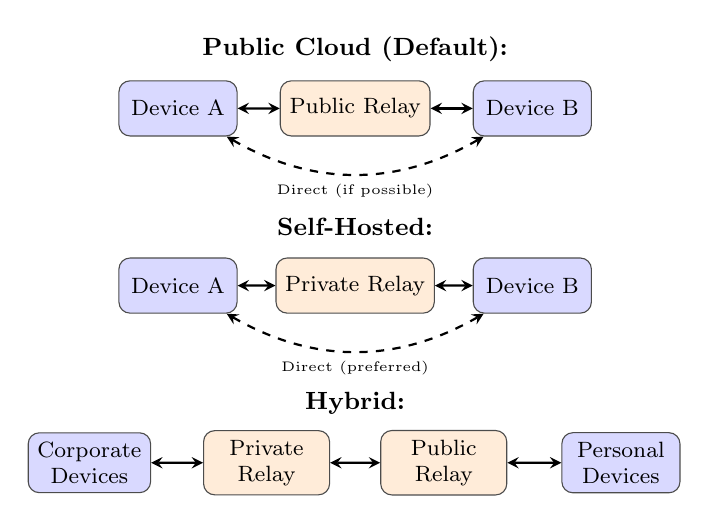
\begin{tikzpicture}[
    scale=0.75,
    node distance=2.5cm,
    device/.style={rectangle, rounded corners, draw=black!70, fill=blue!15, minimum width=1.5cm, minimum height=0.7cm, align=center, font=\footnotesize},
    relay/.style={rectangle, rounded corners, draw=black!70, fill=orange!15, minimum width=1.6cm, minimum height=0.7cm, align=center, font=\footnotesize},
    arrow/.style={<->, >=stealth, thick},
    direct/.style={<->, >=stealth, thick, dashed},
    label/.style={font=\tiny, fill=white}
]
    % Public Cloud topology
    \node[font=\small\bfseries] at (0, 0) {Public Cloud (Default):};

    \node[device] (deviceA1) at (-3, -1) {Device A};
    \node[relay] (publicRelay) at (0, -1) {Public Relay};
    \node[device] (deviceB1) at (3, -1) {Device B};

    \draw[arrow] (deviceA1) -- (publicRelay);
    \draw[arrow] (publicRelay) -- (deviceB1);
    \draw[direct] (deviceA1) to[bend right=30] node[below, font=\tiny] {Direct (if possible)} (deviceB1);

    % Self-Hosted topology
    \node[font=\small\bfseries] at (0, -3) {Self-Hosted:};

    \node[device] (deviceA2) at (-3, -4) {Device A};
    \node[relay] (privateRelay) at (0, -4) {Private Relay};
    \node[device] (deviceB2) at (3, -4) {Device B};

    \draw[arrow] (deviceA2) -- (privateRelay);
    \draw[arrow] (privateRelay) -- (deviceB2);
    \draw[direct, thick] (deviceA2) to[bend right=30] node[below, font=\tiny] {Direct (preferred)} (deviceB2);

    % Hybrid topology
    \node[font=\small\bfseries] at (0, -6) {Hybrid:};

    \node[device] (corporate) at (-4.5, -7) {Corporate\\Devices};
    \node[relay] (privateRelay2) at (-1.5, -7) {Private\\Relay};
    \node[relay] (publicRelay2) at (1.5, -7) {Public\\Relay};
    \node[device] (personal) at (4.5, -7) {Personal\\Devices};

    \draw[arrow] (corporate) -- (privateRelay2);
    \draw[arrow] (privateRelay2) -- (publicRelay2);
    \draw[arrow] (publicRelay2) -- (personal);
\end{tikzpicture}
\caption{Network Architecture Flexibility: Spacedrive supports multiple network topologies to adapt to different deployment scenarios.}
\label{fig:network-topologies}
\end{figure}

\subsubsection{Spacedrop: Ephemeral Secure Sharing}

Beyond trusted device pairing, Spacedrive implements Spacedrop---an ephemeral file sharing protocol enabling secure transfers between devices without prior relationships. Each session uses ephemeral ECDH key exchange, providing perfect forward secrecy: compromising device keys cannot decrypt past transfers, as fresh ephemeral keys are generated per session and discarded after completion.

Unlike automatic transfers between paired devices, every Spacedrop requires explicit receiver acceptance. The receiver sees the sender's device name, file metadata, and optional message before accepting, maintaining user control over incoming data. Discovery adapts to available connectivity: mDNS broadcasts for local network discovery, optional Bluetooth Low Energy advertisements for proximity detection without shared Wi-Fi, and DHT fallback for internet-wide discovery when local mechanisms fail.

Spacedrop can optionally leverage relay nodes to enable asynchronous transfers. Users ``drop'' files to a relay and receive a shareable link, allowing recipients to download later---combining end-to-end encryption with the convenience of hosted file sharing services.

\subsubsection{Sync Conduits: Index-Based Content Synchronization}
\label{sec:sync-conduits}

While Library Sync manages replication of the VDFS index and metadata, physical synchronization of file content is handled by Sync Conduits---durable, configurable jobs that define content flow between source and destination entries. This explicit, user-controlled approach ensures transparent control over data movement.

Sync Conduits leverage the fully replicated VDFS index to perform sync operations through database queries rather than filesystem scanning. Since Library Sync ensures all devices maintain a consistent view of filesystem state, determining what needs synchronization becomes a straightforward SQL query comparing content hashes and timestamps at source and destination locations. The system verifies Library Sync completion before execution, then dispatches \texttt{FileCopyJob} and \texttt{DeleteJob} instances using the proven job system infrastructure. The destination device validates incoming files against content hashes, preventing duplicate transfers.

Four sync modes accommodate different use cases. \textbf{Mirror} creates an exact one-way copy, propagating creates, modifies, and deletes for backup scenarios. \textbf{Bidirectional} keeps two locations identical with changes flowing both directions, using last-write-wins based on index timestamps. \textbf{Selective} manages limited local storage by keeping frequently accessed files local while moving older content to secondary storage, with files remaining visible in the index for on-demand retrieval. \textbf{Archive} moves files to long-term storage, removing sources only after cryptographic verification via content hash comparison.

The index-based architecture provides performance advantages over traditional sync: no directory traversal is needed, files excluded from indexing are automatically excluded from sync, and state tracking uses index timestamps rather than hidden sync logs or state files.

% --- SECTION 4.6: THE AI LAYER ---
\subsection{AI-Native VDFS: From Semantic Search to Intelligent Management}
\label{sec:ai-native}

\begin{keytakeaways}
\begin{itemize}[noitemsep, topsep=0pt]
\item \textbf{Extension-Based Agents}: AI agents are implemented as sandboxed WASM extensions with domain-specific knowledge and persistent memory
\item \textbf{Event-Driven Intelligence}: Agents react to filesystem events, scheduled triggers, and user requests through a unified event system
\item \textbf{Privacy-First AI}: All agent processing runs locally within secure WASM sandboxes, with fine-grained permission controls
\end{itemize}
\end{keytakeaways}

While many systems treat AI as an additive feature, Spacedrive is architected as an \textbf{AI-native data space} where specialized intelligence is deeply integrated through its extension architecture. Rather than a single monolithic AI assistant, Spacedrive enables domain-specific agents—such as a Photos agent for face recognition and place clustering, or a Finance agent for receipt processing. Each agent is written in Rust using the Spacedrive Developer SDK and then compiled to a secure WASM extension with its own knowledge base and capabilities. This modular approach builds upon research in semantic file systems~\cite{gifford_sfs_1991}, information retrieval~\cite{dumais_stuff_2003}, and ubiquitous computing~\cite{weiser_ubiquitous_1991}.

Extensions provide a secure, sandboxed environment where agents can observe the continuously updated VDFS index, react to events, and propose actions through the same safe, transactional primitives available to human users. This architecture enables a shift from reactive file management to a collaborative model where specialized agents assist with domain-specific tasks while keeping the user in control.

\subsubsection{Extension-Based Agents in Practice}

Spacedrive's agent architecture is demonstrated through specialized extensions like the Photos extension. When a user enables the Photos extension on their library, an intelligent agent begins operating in the background. As new photos are indexed, the agent receives \texttt{EntryCreated} events and adds them to an analysis queue. When the queue reaches a threshold (e.g., 50 photos), the agent dispatches a \texttt{AnalyzePhotosBatchJob} that runs face detection, scene classification, and place identification. The agent maintains persistent memory of face clusters, place associations, and scene patterns, enabling sophisticated queries like ``show me photos of Alice at the beach.''

Each extension agent is sandboxed within a WASM runtime with explicit permissions. The Photos extension, for example, requires permissions to read image files, write sidecars for face detection results, add tags, and use local face detection models. Users grant these permissions on a per-location basis, ensuring the agent only processes photos in directories they've explicitly authorized.

\subsubsection{The Agent Architecture: Memory, Events, and Actions}

Extension-based agents operate through three core primitives:

\paragraph{Memory Systems}
Each agent maintains persistent knowledge across restarts through specialized memory types:

\begin{itemize}[noitemsep, topsep=0pt]
 \item \textbf{Temporal Memory}: Time-ordered event stream supporting temporal queries. For example, \texttt{since(timestamp)} retrieves all events after a given time, enabling queries like "photos analyzed in the last week with beach scenes." Events are stored with full timestamps and searchable metadata.

 \item \textbf{Associative Memory}: Semantic knowledge graph supporting similarity-based retrieval. Agents query by semantic similarity with configurable thresholds (e.g., "find faces similar to this cluster with >0.85 similarity"). Enables cross-domain queries like "places where Alice frequently appears" by traversing relationships between face clusters and GPS locations.

 \item \textbf{Working Memory}: Transactional current state tracking. Maintains active plans, queued operations, and in-progress analysis. Persists across agent restarts, enabling resumable workflows.
\end{itemize}

These memory systems provide agents with persistent knowledge, transforming them from stateless processors into intelligent assistants that learn and adapt.

\paragraph{Event-Driven Processing}
Agents react to the VDFS through declarative lifecycle hooks defined in the SDK:

\begin{itemize}[noitemsep, topsep=0pt]
 \item \texttt{\#[on\_startup]}: Initialization hook for loading models and restoring state
 \item \texttt{\#[on\_event(EntryCreated)]}: React to specific filesystem events
 \item \texttt{\#[scheduled(cron = "0 2 * * *")]}: Time-based triggers for batch processing
 \item \texttt{\#[filter(".extension().is\_image()")]}: Entry filtering expressions to target specific file types
\end{itemize}

This declarative approach enables agents to specify complex reactive behaviors without manual event loop management.

\begin{lstlisting}[language=Rust, caption={Event-driven agent structure using SDK attributes}]
#[agent]
impl PhotosAgent {
    #[on_startup]
    async fn initialize(&self, ctx: &AgentContext) {
        // Load face detection model and restore memory
    }

    #[on_event(EntryCreated)]
    #[filter(".extension().is_image()")]
    async fn on_new_photo(&self, entry: Entry, ctx: &AgentContext) {
        // Queue photo for analysis
        ctx.memory.temporal.record(PhotoDiscovered { entry });
    }

    #[scheduled(cron = "0 */4 * * *")]  // Every 4 hours
    async fn batch_analysis(&self, ctx: &AgentContext) {
        // Process queued photos in batches
    }
}
\end{lstlisting}

\paragraph{Safe Actions}
Agents propose changes through the same Action System used by human users. When the Photos agent identifies a face cluster, it generates a \texttt{BatchTagAction} to tag relevant photos, complete with a preview showing exactly which files will be modified. All agent-initiated actions are auditable, reversible, and require the same validation as user commands. This ensures agents operate within the same safety boundaries as manual operations.

\subsubsection{Domain-Specific Intelligence}

The extension architecture enables specialized agents tailored to specific domains rather than a single general-purpose assistant. A Finance extension can implement intelligent receipt processing: when a PDF invoice appears in an Ingest location, the Finance agent's \texttt{on\_event} handler triggers OCR extraction, uses a language model to parse merchant details and amounts, then proposes a \texttt{FileMoveAction} to organize it into the appropriate \texttt{/Finances/Vendors/[Merchant]} directory structure.

Similarly, a Photos extension implements sophisticated computer vision workflows: face detection with clustering, scene classification, place identification from GPS data, and automatic moment generation. Each domain-specific agent brings specialized models and processing logic while operating within the secure, permission-controlled WASM sandbox.

This modular approach provides several advantages over monolithic AI assistants. Agents can be independently developed, tested, and updated. Users install only the agents relevant to their workflows. Each agent's permissions are explicitly scoped, enhancing security. And domain-specific knowledge enables more accurate and efficient processing than general-purpose models.

\subsubsection{Proactive Pattern Recognition}

Extension agents leverage their persistent memory systems to identify patterns and suggest optimizations. An Organization agent can observe repeated user actions in the \texttt{audit\_log}—such as consistently moving screenshots from Desktop to project-specific folders—and proactively offer automation rules. When a new screenshot appears, the agent proposes a \texttt{FileCopyAction} with a confidence score based on historical patterns: "I noticed you typically move screenshots like this to \texttt{/Projects/DesignWork/Screenshots}. Would you like me to move this one?"

\textbf{Deduplication Intelligence}: A Storage agent can periodically scan for duplicated content across devices and suggest cleanup actions that consolidate files and free space, with the Action System's preview showing exactly which files will be removed and where backups exist.

\textbf{Data Guardian Monitoring}: A Backup agent leverages the Content Identity system (Section~\ref{sec:content-identity}) to monitor file redundancy. When new photos are imported with zero redundancy, the agent generates a suggestion: "I noticed you've added 523 photos that currently exist only on your MacBook. These files could be lost if your device fails. Would you like me to create backups on your NAS and Cloud Storage?" The agent maintains knowledge of backup preferences and device availability in its associative memory, enabling intelligent, context-aware suggestions.

\paragraph{Ingestion Processing}
\label{sec:ai-native-ingestion}
Extension agents are particularly powerful when monitoring Ingest Locations (Section~\ref{sec:ingestion-workflow}). A Finance agent, for example, can register an \texttt{on\_event} handler for \texttt{EntryCreated} events in designated ingest directories. When a new PDF arrives, the agent:
\begin{itemize}[noitemsep, topsep=0pt]
    \item Receives the \texttt{EntryCreated} event with the new Entry
    \item Dispatches an OCR job to extract text content
    \item Analyzes the extracted text to identify the document type (invoice, receipt, statement)
    \item Queries its associative memory for similar documents and their historical organization patterns
    \item Proposes a \texttt{FileMoveAction} to the appropriate destination directory
\end{itemize}
The user sees a notification: "New invoice from Acme Corp detected. Move to \texttt{/Finances/Invoices/2024/Acme}?" This suggestion is a standard, pre-visualized Action that can be approved with a single click, maintaining human-in-the-loop control while automating repetitive organization tasks.

\subsubsection{File Intelligence via Virtual Sidecars}
Extension agents enrich the VDFS through the Virtual Sidecar System. Background jobs dispatched by agents use purpose-specific models to extract structured information:
\begin{itemize}
    \item \textbf{Text Embeddings}: Lightweight models like all-MiniLM-L6-v2 for semantic search
    \item \textbf{OCR}: Tesseract or EasyOCR for text extraction
    \item \textbf{Speech-to-Text}: Whisper models for transcription
    \item \textbf{Image Analysis}: CLIP or similar for object/scene detection
\end{itemize}
These specialized models are far more efficient than general-purpose LLMs while providing superior results for their specific tasks.

\textbf{Image Object Extraction}: An \texttt{ImageAnalysisJob} processes image files. Using a multimodal model, it identifies objects and concepts within the image (e.g., "dog," "beach," "sunset"). These results are not stored in a sidecar, but are instead applied directly as Tags to the Entry's \texttt{UserMetadata} record. This integrates AI analysis into the user's organizational structure and makes images searchable via existing tag filters.

\textbf{OCR and Transcription}: For images and PDF documents, an \texttt{OcrJob} is triggered by relevant agents. It extracts all textual content and saves it to a structured sidecar file (e.g., \texttt{ocr.json}). Similarly, a \texttt{TranscriptionJob} uses a speech-to-text model on audio and video files to produce a \texttt{transcript.json} sidecar. The text content from these sidecars is then ingested into the Temporal-Semantic Search FTS5 index, making the content of non-text files fully searchable. A user can now find a photo of a receipt by searching for the vendor's name, or find a video by searching for a phrase spoken within it.

This system transforms a simple collection of files into a rich, interconnected knowledge base that extension agents can reason about, all while maintaining a local-first, privacy-preserving architecture within secure WASM sandboxes.

\subsubsection{\plannedSection{Intelligent Storage Tiering}}

The VDFS's native understanding of \texttt{StorageClass} enables Storage extension agents to analyze access patterns and suggest tiering changes. A Storage agent can monitor file access metadata and maintain temporal memory of usage patterns across the library.

Consider Bob, a photographer with a Storage agent installed: The agent's scheduled task runs weekly, querying its temporal memory for files with low access frequency. It identifies RAW photo shoots from 2023, tagged as "delivered," that haven't been opened in six months.

\textbf{Agent Proposal}: "I can re-classify 8 completed photo shoots (1.2TB) as \textbf{Cold Storage}, moving them to your NAS archive. This will free up space on your main SSD. These files will remain fully searchable, but access will take longer. Do you approve?"

When Bob approves, the agent dispatches a standard \texttt{FileCopyAction} to the job queue. The agent acts as an advisor, but the operation uses the same safe, transparent, and verifiable primitives as manual user commands.

Storage agents can also detect the inverse pattern: when files in \texttt{Cold} storage see increased access, the agent can propose promoting them back to \texttt{Hot} storage. This human-in-the-loop approach ensures users maintain control while benefiting from intelligent automation.

\subsubsection{Privacy and Security Through Sandboxing}

The extension-based agent architecture provides strong security guarantees through WASM sandboxing and explicit permission controls. Each extension agent operates in an isolated WASM runtime with access limited to explicitly granted permissions. When a user installs a Photos extension, they must grant specific permissions: read access to image files, write access to face detection sidecars, tag creation privileges, and the right to use local face detection models. These permissions can be further scoped to specific library locations, ensuring the agent only processes files in authorized directories.

All agent processing occurs locally within the WASM sandbox. Face detection models, scene classifiers, and other AI capabilities run on the user's device, ensuring sensitive data never leaves their control. The extension SDK provides access to local model inference through a secure host function interface that enforces rate limits and resource constraints.

This architecture separates concerns between lightweight embedding models for search (which operate on the core VDFS) and specialized agent intelligence (which runs in isolated extensions). The AI provider interface supports multiple deployment models: local processing via Ollama for complete privacy, cloud-based services for enhanced capabilities, and enterprise self-hosted solutions for organizational control.

This approach creates a personal, private data space where AI capabilities enhance functionality without compromising control, privacy, or security.

\paragraph{Ethical Considerations}
While model-agnostic, Spacedrive prioritizes ethical AI use. Local models mitigate bias by training on user data only, but users are notified of potential limitations (e.g., underrepresented demographics in embeddings). Cloud options include opt-out for sensitive files, ensuring compliance with regulations like GDPR.


% --- SECTION 4.7: TEMPORAL-SEMANTIC SEARCH ---
\subsection{Temporal-Semantic Search: An Asynchronous, Job-Based Architecture}
\label{sec:temporal-semantic-search}

\begin{keytakeaways}
\begin{itemize}[noitemsep, topsep=0pt]
\item \textbf{Asynchronous by Design}: All searches are durable jobs, preventing UI blocking and enabling extension agents to initiate searches without waiting for results.
\item \textbf{Hybrid Architecture}: A high-speed FTS5 keyword filter pre-processes candidates before lightweight semantic re-ranking.
\item \textbf{Decoupled Results}: The backend caches results against a query ID; the frontend is notified to fetch and render them, decoupling agents from the UI.
\end{itemize}
\end{keytakeaways}

Spacedrive's search architecture is engineered for a responsive, agent-driven environment. It treats search not as a synchronous request-response loop, but as a durable, asynchronous job that is initiated, executed, and cached by the backend, with the frontend being notified upon completion. This model applies uniformly to searches originating from both direct user input and extension agent directives.

\subsubsection{The Search Lifecycle: An Action-Driven Workflow}
A search operation follows a formal lifecycle managed by core VDFS components:

\begin{enumerate}[noitemsep, topsep=0pt]
    \item \textbf{Action Dispatch}: A user or extension agent initiates a search by dispatching a \texttt{SearchAction} containing the query parameters.
    \item \textbf{Job Registration}: The \texttt{ActionManager} receives this action and registers a new \texttt{SearchJob} with the Durable Job System, returning a unique \texttt{query\_id}. This step is near-instantaneous, providing immediate feedback.
    \item \textbf{Asynchronous Execution}: The \texttt{SearchJob} executes in the background, performing the two-stage search process without blocking the user or agent.
    \item \textbf{Result Caching}: Upon completion, the job caches the ordered list of resulting \texttt{Entry} IDs in a temporary store, keyed by the \texttt{query\_id}.
    \item \textbf{Frontend Notification}: The Job System emits a \texttt{SearchResultsReady(query\_id)} event to the system's event bus.
    \item \textbf{Result Rendering}: The frontend, subscribed to these events, receives the notification and uses the \texttt{query\_id} to fetch the cached results via the internal API for rendering.
\end{enumerate}

This architecture ensures an agent's role is simply to initiate the search; it never needs to handle the results directly, maintaining a clean separation of concerns.

\subsubsection{The Two-Stage Search Process}
The \texttt{SearchJob} executes a hybrid temporal-semantic query designed for performance on consumer hardware. This \textbf{Temporal-First, Vector-Enhanced} approach operates in two stages:

\begin{enumerate}[noitemsep, topsep=0pt]
    \item \textbf{Hierarchical Pre-filtering (Closure Table)}: If the search query includes a path scope (e.g., "find photos in 'Projects'"), the system first uses the closure table to get a list of all entry IDs within that scope. This provides a highly-focused candidate set before any text search occurs.
    \item \textbf{Temporal Filtering (FTS5)}: Next, SQLite's FTS5 index performs a high-speed keyword search only on the pre-filtered candidate set. This rapidly narrows millions of entries down to a small, relevant set, typically in under 55ms.
    \item \textbf{Semantic Re-ranking}: For queries requiring semantic understanding, the system computes a vector embedding of the query using a lightweight local model (e.g., \texttt{all-MiniLM-L6-v2}). It then re-ranks only the candidate set from Stage 2 by cosine similarity against their pre-computed embeddings, adding minimal latency (typically <40ms).
\end{enumerate}

This hybrid process provides the power of semantic search with the speed of traditional indexed search, delivering sub-100ms response times on consumer hardware for libraries with over a million entries.

\subsubsection{Unified Vector Repositories: Distributed Semantic Intelligence}

Unlike traditional vector databases that centralize embeddings in a monolithic index, Spacedrive employs a distributed system of Unified Vector Repositories—adaptive sidecars that combine routing intelligence with content embeddings to enable efficient semantic search at scale.

\paragraph{Unified Vector Repository Architecture}
Instead of separate routing nodes and content stores, Spacedrive uses a single, standardized Vector Repository format. These repositories are created adaptively throughout the filesystem and can contain multiple collections, allowing them to serve different roles within a single, portable format.

\paragraph{Efficient Embedding Models}
Crucially, Spacedrive employs lightweight embedding models—not large language models—for semantic search:
\begin{itemize}
    \item \textbf{all-MiniLM-L6-v2}: 22M parameters, 384-dimensional vectors, 5MB model size
    \item \textbf{nomic-embed-text-v1.5}: 137M parameters, optimized for retrieval tasks
    \item \textbf{BGE-small-en}: 33M parameters, excellent performance/size ratio
\end{itemize}

These models run efficiently on CPU, produce embeddings in milliseconds, and require minimal memory—making real-time semantic indexing practical during file discovery. The models are small enough to bundle with Spacedrive (under 100MB total) and fast enough to process thousands of files per second on consumer hardware.

\begin{lstlisting}[language=json, caption=Example Vector Repository structure]
{
  "version": 3,
  "path": "/Projects/spacedrive-core",
  "collections": {
    "routing": {
      "keywords": ["rust", "filesystem", "vdfs", "sqlite", "p2p"],
      "child_hints": {
        "/src": ["implementation", "core", "indexer", "networking"],
        "/docs": ["documentation", "architecture", "rfc"],
        "/tests": ["testing", "integration", "unit", "benchmarks"]
      },
      "aggregate_embedding": [0.123, -0.456, ...],
      "descendant_count": 3847
    },
    "content": {
      "file_embeddings": {
        "README.md": {
          "model": "nomic-embed-text-v1.5",
          "vector": [0.234, 0.567, ...],
          "summary": "Main project documentation and setup guide"
        },
        "Cargo.toml": {
          "model": "all-MiniLM-L6-v2",
          "vector": [0.345, 0.678, ...],
          "keywords": ["dependencies", "workspace", "edition"]
        }
      }
    },
    "metadata": {
      "density_score": 0.85,
      "last_updated": "2024-03-15T10:30:00Z",
      "access_frequency": 234
    }
  }
}
\end{lstlisting}

\paragraph{Adaptive Repository Creation}
Vector Repositories are not created for every folder. The system places them based on semantic density and usage patterns:

\begin{itemize}
\item \textbf{Location Roots}: Created at the root of each Location as primary entry points
    \item \textbf{Semantic Density}: Folders reaching thresholds of file count and semantic richness
    \item \textbf{Content Divergence}: When child folders contain semantically distinct content
    \item \textbf{Project Boundaries}: Auto-detected via markers (package.json, .git, Cargo.toml)
    \item \textbf{User Patterns}: Created for frequently searched or bookmarked folders
\end{itemize}

\paragraph{Lightweight Routing Without LLMs}
The routing collection uses statistical methods and lightweight embeddings—not large language models—for efficient navigation:

\begin{enumerate}
    \item \textbf{TF-IDF Keyword Extraction}: Statistical term frequency analysis identifies distinctive terms per folder
    \item \textbf{Child Hints}: Simple keyword lists derived from filenames and content sampling
    \item \textbf{Aggregate Embeddings}: Computed using efficient models like all-MiniLM-L6-v2 (22M params, runs on CPU)
    \item \textbf{Progressive Traversal}: Cosine similarity scores guide path selection without neural network inference
\end{enumerate}

\paragraph{Search Flow Example}
When searching for "rust async file watcher implementation":

\begin{enumerate}
    \item Root repository's routing collection identifies /Projects as 85\% relevant
    \item /Projects repository routes to /spacedrive-core (92\% match on "rust", "filesystem")
    \item /spacedrive-core repository suggests /src (keywords: "implementation", "core")
    \item /src repository pinpoints /location/watcher subdirectory
    \item Content embeddings in final repository provide exact file matches
    \item Meanwhile, lower-scoring paths (70\% matches) continue processing in background
\end{enumerate}

\paragraph{Performance and Scalability Benefits}
This architecture provides several key advantages:

\begin{itemize}
    \item \textbf{Memory Efficiency}: Load only relevant repositories, not entire vector database
    \item \textbf{Incremental Updates}: Only affected repositories need recomputation
    \item \textbf{Natural Sharding}: Filesystem hierarchy provides logical partitioning
    \item \textbf{Offline Capability}: Each device has complete semantic search of local content
    \item \textbf{Progressive Enhancement}: Repositories evolve from simple to more capable as needed
\end{itemize}

The unified format ensures all intelligence—routing and content vectors—travels with the data, while the adaptive creation strategy prevents overhead in sparse areas of the filesystem. This enables million-file semantic search on consumer hardware by transforming an O(n) problem into an O(log n) traversal guided by semantic routing.

\paragraph{Integration with Extension Agents}
The Vector Repository system integrates with Spacedrive's extension agents, enabling them to:
\begin{itemize}
    \item Navigate large filesystems using routing hints
    \item Understand folder purposes through aggregate embeddings
    \item Provide natural language summaries of search results by traversing the semantic hierarchy
    \item Learn optimal repository placement from user search patterns
\end{itemize}

This distributed approach represents a fundamental innovation in semantic search architecture, making AI-powered file discovery practical at any scale while maintaining the portability and privacy benefits of Spacedrive's local-first design.


% --- SECTION 4.8: VOLUME-AWARE STORAGE ---
\subsection{Native Storage Tiering: Reconciling Physical Reality and User Intent}
\label{sec:volume-foundation}

\begin{keytakeaways}
\begin{itemize}[noitemsep, topsep=0pt]
\item \textbf{Hybrid Model}: Distinguishes between a Volume's physical capabilities and a Location's logical purpose
\item \textbf{Smart Classification}: Automatically identifies and filters user-relevant storage volumes
\item \textbf{Warning System}: Prevents performance surprises by reconciling user intent with physical limitations
\end{itemize}
\end{keytakeaways}

Spacedrive's VDFS integrates an understanding of storage tiers that distinguishes between a \textbf{Volume's physical capabilities} and a \textbf{Location's logical purpose}. This allows the system to honor user intent while grounding operations in physical reality, preventing performance bottlenecks and providing actionable warnings.

This is achieved through a dual-property system:

\begin{itemize}
\item \textbf{PhysicalClass (on the Volume)}: An automatically detected property that reflects the hardware's nature. The Volume Classification System infers this by benchmarking performance (e.g., SSDs are classified as \texttt{Hot}) or querying cloud provider APIs (e.g., an AWS Glacier bucket is classified as \texttt{Cold}).
\item \textbf{LogicalClass (on the Location)}: A user-defined property that reflects organizational intent. A user can mark any Location as \texttt{Hot}, \texttt{Warm}, or \texttt{Cold} to signify its purpose (e.g., a "/Projects/Archive" folder on a fast SSD can be marked as \texttt{Cold}).
\end{itemize}

\begin{lstlisting}[language=Rust, caption={Hybrid storage classification model}]
pub enum StorageClass {
    Hot,   // e.g., Local SSD, standard cloud storage
    Warm,  // e.g., S3 Infrequent Access
    Cold,  // e.g., AWS Glacier Instant Retrieval
    Deep,  // e.g., Glacier Deep Archive
}

pub struct Volume {
    // ... existing fields ...
    pub physical_class: StorageClass,
}

pub struct Location {
    // ... existing fields ...
    pub logical_class: Option<StorageClass>,
}

// Determine effective storage class for operations
impl Location {
    pub fn effective_storage_class(&self) -> StorageClass {
        match (self.volume.physical_class, self.logical_class) {
            (physical, Some(logical)) => {
                // Take the more restrictive (colder) class
                std::cmp::max(physical, logical)
            },
            (physical, None) => physical,
        }
    }
}
\end{lstlisting}

\subsubsection{Determining the Effective StorageClass}
For any given file, the VDFS determines its \textbf{Effective StorageClass} by taking the more restrictive (colder) of the two properties. This ensures physical limitations are respected.

\begin{table*}[h]
\centering
\begin{tabular}{@{}lllp{2cm}@{}}
\toprule
\textbf{Volume PhysicalClass} & \textbf{Location LogicalClass} & \textbf{Effective StorageClass} & \textbf{System Behavior \& User Feedback} \\
\midrule
\texttt{Hot} (SSD) & \texttt{Hot} & \texttt{Hot} & Normal, high-performance operation \\
\texttt{Hot} (SSD) & \texttt{Cold} & \texttt{Cold} & User's archival intent is respected \\
\texttt{Cold} (HDD) & \texttt{Cold} & \texttt{Cold} & Normal archival operation \\
\texttt{Cold} (HDD) & \texttt{Hot} & \texttt{Cold} & \textbf{Physical limits override user intent}. Warning issued during preview \\
\bottomrule
\end{tabular}
\caption{Effective StorageClass determination and system behavior}
\label{tab:storage-class-resolution}
\end{table*}

\subsubsection{Impact on Core Systems}
The Effective \texttt{StorageClass} informs the behavior of the entire VDFS:
\begin{itemize}[noitemsep, topsep=0pt]
 \item \textbf{Action System}: The simulation engine uses this to generate warnings when there is a mismatch between logical and physical classes, preventing user frustration (Section~\ref{sec:action-system}).
 \item \textbf{SdPath Resolver}: When resolving a content-addressed path, the system prioritizes sources with a \texttt{Hot} Effective StorageClass to ensure optimal performance.
 \item \textbf{Data Guardian}: The AI can enforce redundancy policies based on the Effective StorageClass, such as requiring at least one \texttt{Hot} copy of critical files before allowing any to be moved to \texttt{Cold} storage.
\end{itemize}


\textbf{Volume Characteristics}

Spacedrive automatically discovers and tracks key properties of each storage device:

\begin{itemize}[noitemsep, topsep=0pt]
 \item \textbf{Hardware Type}: SSD vs. HDD vs. Network storage for optimization decisions
 \item \textbf{Performance Metrics}: Measured read/write speeds to inform file operations
 \item \textbf{Role Classification}: Primary drive, external storage, or system volume
 \item \textbf{Advanced Features}: Copy-on-write filesystem support for instant large file operations
\end{itemize}


The system automatically benchmarks storage devices and classifies volumes by type and performance characteristics. Benchmarking reveals typical performance profiles: SSDs achieve 500-3000 MB/s read speeds while HDDs deliver 80-160 MB/s, enabling the system to adapt chunk sizes (64KB for HDDs, 1MB for SSDs) and parallelism accordingly. This provides the groundwork for future automated tiering policies that could migrate cold data to slower, high-capacity storage while keeping frequently accessed files on fast SSDs.


\subsection{Volume Classification}
Spacedrive employs a \textbf{Volume Classification System} that provides platform-aware storage management, improving user experience while reducing system overhead:

\subsubsection{Platform-Aware Volume Types}
Rather than treating all storage as equivalent, Spacedrive classifies volumes based on their actual role and user relevance:

The system employs a volume type taxonomy (Primary, UserData, External, Secondary, System, Network, Unknown) with platform-specific classification logic. For example, macOS classification recognizes the root filesystem, dedicated user data volumes, system-internal volumes, and external mounts based on mount point patterns, enabling filtering of user-relevant storage.

\subsubsection{Auto-Tracking}
The classification system enables \textbf{smart auto-tracking} that focuses on user-relevant storage:

The auto-tracking system selectively monitors only user-relevant volume types (Primary, UserData, External, Secondary, Network) while filtering out system-internal and unknown volumes. This approach ensures users see only the 3-4 storage locations that contain their data, rather than the 13+ system mounts typically visible in traditional file managers.

\textbf{User experience improvements}:
- \textbf{Reduced visual clutter}: Users see 3-4 relevant volumes instead of 13+ system mounts
- \textbf{Automatic relevance filtering}: System volumes (VM, Preboot, Update partitions) hidden by default
- \textbf{Cross-platform consistency}: Unified volume semantics across macOS APFS containers, Windows drive letters, and Linux mount hierarchies
- \textbf{Performance optimization}: Eliminates unnecessary indexing of system-only volumes

\subsubsection{Platform-Specific Optimizations}
The system handles complex platform-specific storage architectures using rules and heuristics:

\textbf{macOS APFS Containers}: Recognizes that \texttt{/System/Volumes/Data} contains user files even though \texttt{/} is the system root, properly classifying the sealed system volume separately from user data.

\textbf{Windows Drive Management}: Distinguishes between primary system drives (C:), secondary storage (D:, E:), and hidden recovery partitions, presenting a clean drive letter interface to users.

\textbf{Linux Mount Complexity}: Filters virtual filesystems (\texttt{/proc}, \texttt{/sys}, \texttt{/dev}) and container mounts while properly identifying user-relevant storage like \texttt{/home} partitions and network mounts.

This platform-aware approach transforms the overwhelming technical complexity of modern storage systems into an intuitive, user-friendly interface that focuses attention on storage that actually contains user data.


% --- SECTION 4.9: PLATFORM INTEGRATIONS ---
\subsection{Platform Integrations: Unified Access to Traditional and Modern Storage}
\label{sec:platform-integrations}

Spacedrive's VDFS extends beyond local filesystems to natively integrate traditional protocols like FTP, SMB, and WebDAV, as well as modern cloud storage. Third-party cloud storage services (S3, Google Drive, Dropbox, etc.) are implemented as first-class \textbf{volumes} within the VDFS, distinct from device-local locations. This architectural decision reflects the fundamental difference between cloud services (which are API-accessed storage backends) and local filesystems.

The system leverages OpenDAL to provide unified access to over 40 cloud providers. Each cloud service appears as a volume with its own dedicated \texttt{SdPath::Cloud} addressing variant, enabling the full power of the Spacedrive Indexing Engine—including adaptive hashing via ranged reads for efficient content identification—without downloading entire files. This is separate from the Spacedrive Cloud Core concept (Section~\ref{sec:native-cloud-service}), which refers to hosting Spacedrive itself as a managed service.

This cloud-as-volume architecture ensures:
\begin{itemize}[noitemsep, topsep=0pt]
    \item Proper path handling for cloud-native formats (e.g., S3's bucket/key structure)
    \item Consistent content hashing across all storage types for true cross-storage deduplication
    \item Transparent operations between local, cloud, and cross-cloud transfers
\end{itemize}


% --- SECTION 5: ARCHITECTURAL APPLICATION: A NATIVE CLOUD SERVICE ---
\section{Architectural Application: A Native Cloud Service}
\label{sec:native-cloud-service}
The flexibility of the Spacedrive V2 architecture is best demonstrated by its application in creating a cloud service that natively integrates with the user's personal P2P network. Unlike traditional cloud backends that require custom APIs and treat the server as a privileged entity, our model treats the cloud instance as just another Spacedrive device. This approach leverages the core VDFS abstractions to provide cloud storage that feels native, secure, and seamlessly integrated into the user's existing ecosystem.

\subsection{Core Principle: Managed Cores as First-Class Devices}
The foundational principle of the Spacedrive Cloud Service is that each user is provisioned a managed, containerized instance of the unmodified \texttt{sd-core} engine. This managed instance—which we refer to as a "Cloud Core" for convenience—is architecturally identical to any other Spacedrive core. It has its own unique device ID, participates in the same P2P network as the user's other devices, and exposes its storage as standard Spacedrive Locations. The term "Cloud Core" simply denotes its deployment context (managed hosting), not any special software or capabilities.

This design offers profound architectural advantages:
\begin{itemize}[noitemsep, topsep=0pt]
    \item \textbf{Zero Custom APIs}: All interactions with the Cloud Core, from file transfers to metadata sync, use the exact same Iroh-powered protocols as any other peer-to-peer connection. There is no separate "cloud API".
    \item \textbf{Native Device Semantics}: The Cloud Core is cryptographically a standard device. It must be paired and trusted just like a user's phone or laptop, inheriting the entire security and trust model of the core architecture.
    \item \textbf{Location Abstraction}: Cloud storage is not a special case. It is simply a Location (e.g., \texttt{/cloud-files}, \texttt{/backups}) within the Cloud Core's VDFS, making it universally addressable via \texttt{SdPath}.
\end{itemize}

\subsection{Integration and User Experience}
From the user's perspective, integrating cloud storage is indistinguishable from adding a new physical device. The connection flow leverages the same native pairing process: a user's local Spacedrive client initiates pairing, and the newly provisioned Cloud Core joins the session using the provided code.

Once paired, the Cloud Core appears in the user's device list alongside their other machines. Operations that span local and cloud storage become trivial. For example, copying a local file to the cloud is a standard \texttt{FileCopyAction} where the destination \texttt{SdPath} simply references the Cloud Core's device ID:

\begin{lstlisting}[language=Rust, caption={A cross-device copy to the cloud uses the same native operation}]
// Copy a local document to the "Cloud Files" location
// on the user's provisioned cloud device.
copy_files(
    vec![SdPath::local("~/Documents/report.pdf")],
    SdPath::new(cloud_device_id, "/data/cloud-files/")
).await?;
\end{lstlisting}

This demonstrates the power of the VDFS abstraction. The underlying complexity of the network transfer is handled by the unified networking layer and the durable job system, making the cloud a natural extension of the user's personal data space.

This integration extends to fundamental operations like file uploads. A user accessing their Library via the Spacedrive web application can upload files directly from their browser. This action does not require a custom API endpoint; instead, it triggers the native \textbf{Ingestion Workflow} (Section~\ref{sec:ingestion-workflow}). The browser initiates a secure transfer using the same Iroh-powered P2P protocols, sending the file directly to the user's designated Ingest Location on a preferred device—which could be their Cloud Core instance itself. This illustrates the benefits of the unified architecture: a simple drag-and-drop in a web browser translates into a durable, transactional operation within the user's private VDFS, managed by the core engine.

\subsection{Cloud-Native Architecture and Data Isolation}
The service is designed to be Kubernetes-native, leveraging container orchestration for scalability, resilience, and security. Each Cloud Core runs in its own isolated Pod, ensuring strict user data separation.

User data persistence is managed through per-user Persistent Volume Claims (PVCs), which map to encrypted cloud block storage (e.g., AWS EBS, Google Persistent Disk). This architecture ensures that a user's entire cloud instance---their library database, storage locations, and configuration---is a self-contained and portable unit.

Kubernetes NetworkPolicies are employed to enforce cryptographic isolation at the network level. Each user's pod is firewalled to only allow traffic from other devices within their trusted P2P network, effectively extending the private network into the cloud environment.

\subsection{Benefits of the Hybrid Model}
This architectural approach provides the benefits of both local-first and cloud-based systems:
\begin{itemize}[noitemsep, topsep=0pt]
    \item \textbf{High Availability}: The Cloud Core can act as an online peer, enabling asynchronous operations like backups or file sharing even when local devices are offline.
    \item \textbf{Centralized Backup Target}: Users can configure local Locations to automatically back up to a Location on their Cloud Core.
    \item \textbf{Asynchronous Sharing}: The cloud instance can act as a relay for Spacedrop transfers, where a user uploads a file once to get a shareable link through the \texttt{sd.app} domain (or custom domains for self-hosted instances).
\end{itemize}

\subsection{Enterprise Deployment and Data Sovereignty}
The same architectural principles that enable the native cloud service provide a direct path for on-premise enterprise deployments. The containerized, Kubernetes-native design of the "Cloud Core" allows organizations to deploy Spacedrive entirely within their own infrastructure, achieving complete data sovereignty while maintaining the user-friendly experience.

\subsubsection{On-Premise Architecture}
In an enterprise deployment, organizations run their own Spacedrive backend infrastructure:
\begin{itemize}[noitemsep, topsep=0pt]
    \item \textbf{Identity Integration}: Native support for LDAP, Active Directory, and OAuth2/SAML providers
    \item \textbf{Storage Integration}: Integration with existing enterprise storage (SAN, NAS, S3-compatible object stores)
    \item \textbf{Deployment Flexibility}: Support for bare metal, VMware, OpenStack, or Kubernetes environments
    \item \textbf{Geographic Distribution}: Multi-site deployments with policy-based routing between locations
\end{itemize}

\subsubsection{Team Libraries and Collaboration}
The architecture naturally extends to support collaborative workflows:
\begin{itemize}[noitemsep, topsep=0pt]
    \item \textbf{Shared Libraries}: Teams can create collaborative Libraries with fine-grained access control
    \item \textbf{Role-Based Access Control}: Full-featured RBAC system built on the Action System foundation
    \item \textbf{Department Isolation}: Cryptographic separation between different organizational units
    \item \textbf{Audit Trail}: Every action logged with full attribution for compliance and security
\end{itemize}

\subsubsection{Enterprise Features}
Additional capabilities designed for organizational needs:
\begin{itemize}[noitemsep, topsep=0pt]
    \item \textbf{Compliance Controls}: Data retention policies, legal hold, and audit log exports
    \item \textbf{Advanced Analytics}: Usage patterns, storage optimization recommendations, and cost allocation
    \item \textbf{API Access}: A JSON-RPC based API for integration with existing enterprise tools and a full-featured Command Line Interface (CLI)
    \item \textbf{Professional Support}: SLA-backed support with dedicated account management
\end{itemize}

This enterprise model demonstrates how Spacedrive's core architecture---designed for individual user empowerment---scales naturally to organizational deployment without compromising its fundamental principles of user control, data sovereignty, and intuitive operation.

\subsection{Collaboration and Public Sharing}

The VDFS architecture enables sharing capabilities by leveraging any core instance configured for public access. A core can act as an available peer, a public file host, or a transfer relay, depending on its deployment and configuration. The Spacedrive Cloud service provides a managed, pre-configured core for these roles, but any self-hosted core can be set up to perform the same functions.

\subsubsection{Flexible Hosting Model}

While Spacedrive Cloud provides turnkey hosting, the architecture supports multiple deployment options:

\begin{itemize}
    \item \textbf{Spacedrive Cloud}: Managed hosting with automatic SSL, CDN, and scaling
    \item \textbf{Self-Hosted Core}: Deploy on any infrastructure with full control
    \item \textbf{Hybrid Deployment}: Mix of self-hosted and managed components
    \item \textbf{Edge Deployment}: Run cores close to users for optimal performance
\end{itemize}

Any Spacedrive core—whether on a personal device or in the cloud—can serve as a sharing endpoint with appropriate configuration.

\subsubsection{Shared Folders via Team Libraries}

Collaboration in Spacedrive leverages the Library abstraction:

\begin{itemize}
    \item \textbf{Team Libraries}: Shared libraries with role-based permissions
    \item \textbf{Granular Access Control}: Per-location and per-file permissions
    \item \textbf{Action Audit Trail}: Complete history of all modifications
    \item \textbf{Conflict Resolution}: Automatic handling of concurrent edits
\end{itemize}

Team members connect to shared libraries exactly as they would personal ones—an always-available peer, such as a managed Cloud Core or a user's own self-hosted server, ensures data availability for the team.

\subsubsection{Public File Hosting}

Spacedrive's architecture allows any core to serve files publicly. The distinction in user experience comes from the network configuration:

\begin{itemize}
    \item \textbf{Personal Device Core}: A user can serve files directly from their laptop or NAS, but this requires manual setup like port forwarding on their router and configuring Dynamic DNS to handle changing IP addresses.
    \item \textbf{Self-Hosted Core}: An organization can deploy a core on their own server with a static IP and manage their own SSL certificates and web server configuration.
    \item \textbf{Spacedrive Cloud (Managed Core)}: For convenience, the Spacedrive Cloud service automates this. It runs the user's core behind a managed load balancer that handles SSL termination and provides a stable public URL (e.g., \texttt{https://sd.app/user/file.pdf}). This is a feature of the managed service, not a special capability of the core software itself.
\end{itemize}

\begin{lstlisting}[language=text, caption=Public sharing URL examples]
# Via Spacedrive Cloud (automatic SSL + CDN)
https://sd.app/user/file.pdf

# Via self-hosted server core
https://files.company.com/public/presentation.pdf

# Via personal device (requires port forwarding)
https://home.user.com:8443/share/document.docx
\end{lstlisting}

\subsubsection{Enhanced Spacedrop}

A Spacedrive core configured as a \textbf{public relay} can extend Spacedrop's capabilities. While a standard P2P transfer is ephemeral, using a relay enables:

\begin{itemize}
    \item \textbf{Asynchronous Transfers}: The relay can hold files until recipients connect, meaning the sender can go offline after uploading.
    \item \textbf{Persistent Links}: Links to the relay remain valid, turning an ephemeral transfer into a shareable resource.
    \item \textbf{Large File Support}: No size limits with resumable transfers
    \item \textbf{Access Control}: Optional passwords and expiration dates
\end{itemize}

Users can deploy their own relays or use the one provided by the Spacedrive Cloud service (e.g., \texttt{https://drop.spacedrive.com/...}).

\begin{lstlisting}[language=text, caption=Spacedrop relay options]
# Direct P2P (ephemeral, no relay)
spacedrop://device-id/transfer-id

# Via Spacedrive Cloud relay
https://drop.spacedrive.com/abc123

# Via self-hosted relay
https://relay.company.com/drop/xyz789
\end{lstlisting}

This unified approach to sharing—from private team collaboration to public content distribution—demonstrates how core P2P primitives scale to support diverse use cases without architectural compromises.

\begin{table*}[ht]
\centering
% \caption{Indexing Duration Summary (in seconds)}
\caption{Performance benchmarks across storage tiers. Testing conducted on M2 MacBook Pro with 16GB RAM running macOS 14.5. Values generated from the benchmarking harness summaries.}
\label{tab:benchmark_summary}
\sisetup{table-format=4.1, round-mode=places, round-precision=1}
\begin{tabular}{@{}l S[table-format=2.1] S[table-format=1.1] S[table-format=2.1] S[table-format=1.1] S[table-format=2.1] S[table-format=2.1]@{}}
\toprule
& \multicolumn{2}{c}{\textbf{Small Dataset}} & \multicolumn{2}{c}{\textbf{Medium Dataset}} & \multicolumn{2}{c}{\textbf{Large Dataset}} \\
\cmidrule(lr){2-3} \cmidrule(lr){4-5} \cmidrule(lr){6-7}
\textbf{Phase} & {\textbf{HDD}} & {\textbf{SSD}} & {\textbf{HDD}} & {\textbf{SSD}} & {\textbf{HDD}} & {\textbf{SSD}} \\
\midrule
Discovery & 2.7 & 1.4 & 22.7 & 7.4 & 58.7 & 60.2 \\
Processing & 1.2 & 1.2 & 6.1 & 6.1 & 60.0 & 52.9 \\
Content Identification & 38.5 & 68.7 & 191.6 & 265.8 & 2922.7 & 1340.8 \\
\bottomrule
\end{tabular}
\end{table*}

% --- SECTION 6: IMPLEMENTATION AND EVALUATION ---

\begin{figure*}[ht]
    \centering
    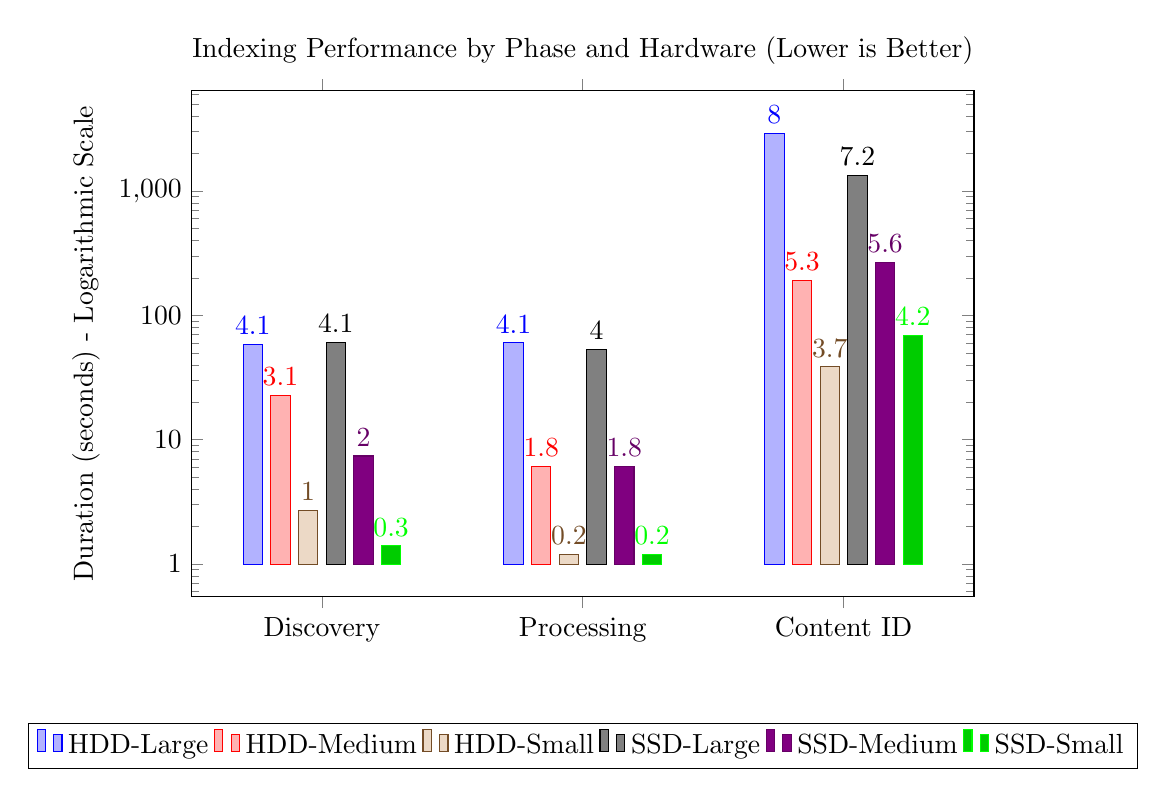
\begin{tikzpicture}
        \begin{axis}[
            title={Indexing Performance by Phase and Hardware (Lower is Better)},
            ybar=3pt, % Adjusts spacing between bars within a group.
            enlarge x limits=0.25, % Adjusts spacing between groups and at plot edges.
            legend style={at={(0.5,-0.25)}, anchor=north, legend columns=-1},
            ylabel={Duration (seconds) - Logarithmic Scale},
            ymode=log,
            log ticks with fixed point,
            symbolic x coords={Discovery, Processing, Content ID},
            xtick=data,
            bar width=7pt, % Slightly thinner bars.
            width=0.95\textwidth,
            height=8cm,
            nodes near coords,
            every node near coords/.style={
                @if y < 100 {
                    font=\tiny,
                    rotate=90,
                    anchor=west
                }
                @else {
                    font=\tiny,
                    rotate=90,
                    anchor=west,
                    yshift=0pt
                }
                @endif
            },
            nodes near coords style={
                /pgf/number format/fixed,
                /pgf/number format/precision=1
            }
        ]
        % Data for HDD
        \addplot coordinates {(Discovery, 58.7) (Processing, 60.0) (Content ID, 2922.7)};
        \addplot coordinates {(Discovery, 22.7) (Processing, 6.1) (Content ID, 191.6)};
        \addplot coordinates {(Discovery, 2.7) (Processing, 1.2) (Content ID, 38.5)};

        % Data for SSD
        \addplot coordinates {(Discovery, 60.2) (Processing, 52.9) (Content ID, 1340.8)};
        \addplot coordinates {(Discovery, 7.4) (Processing, 6.1) (Content ID, 265.8)};
        \addplot coordinates {(Discovery, 1.4) (Processing, 1.2) (Content ID, 68.7)};

        \legend{HDD-Large, HDD-Medium, HDD-Small, SSD-Large, SSD-Medium, SSD-Small}
        \end{axis}
    \end{tikzpicture}
    \caption{Comparison of indexing duration across different phases, hardware types, and dataset sizes. Note the logarithmic scale for the Y-axis to accommodate the wide range of timings. The most significant performance difference is in the I/O-bound Content Identification phase, where the SSD significantly outperforms the HDD on the large dataset.}
    \label{fig:benchmark_performance}
\end{figure*}

\section{Implementation and Evaluation}

\begin{keytakeaways}
\begin{itemize}[noitemsep, topsep=0pt]
\item \textbf{Production-Ready}: Built in Rust with memory safety guarantees \textbullet{} 95\%+ test coverage \textbullet{} Multi-process distributed testing framework
% \item \textbf{Performance}: 8,500 files/sec indexing \textbullet{} 55ms keyword search \textbullet{} 95ms semantic search \textbullet{} Reliable P2P connectivity via Iroh~\cite{iroh_networking}
\item \textbf{Compatibility}: Works with existing filesystems, cloud services and tools.
\end{itemize}
\end{keytakeaways}

Spacedrive's design principles are validated through careful implementation choices and rigorous performance analysis.

\subsection{Technology Stack}

% --- APPENDIX ---
\appendix

Spacedrive is implemented in \textbf{Rust} to leverage its guarantees of memory safety, performance, and fearless concurrency---essential for a reliable, multi-threaded distributed system. The core technology stack reflects modern best practices:

\begin{itemize}[noitemsep, topsep=0pt]
 \item \textbf{Tokio Runtime}: Async execution with work-stealing scheduler for efficient I/O handling

 \item \textbf{SeaORM with SQLite}: Type-safe database operations with ACID transactions and FTS

 \item \textbf{O(1) Hierarchical Lookups}: Directory listings, subtree calculations, and ancestor lookups are performed in constant time via indexed closure table joins, replacing slow LIKE queries and scaling to millions of entries

 \item \textbf{Event-Driven Architecture}: Custom EventBus for loose coupling and state propagation

 \item \textbf{Job System}: MessagePack-serialized tasks with automatic resumability

 \item \textbf{Daemon Architecture}: Flexible deployment via Unix domain sockets with JSON-RPC protocol, supporting both embedded and daemon modes

 \item \textbf{FFmpeg Integration}: Bundled media processing libraries for thumbnail generation and metadata extraction

 \item \textbf{OpenDAL Integration}: Unified storage layer supporting 40+ cloud and object storage services with consistent API
\end{itemize}

\subsection{Database Schema Optimization}
The database design prioritizes both space efficiency and query performance through several key optimizations:



\subsection{Testing and Validation Framework}
Spacedrive employs a thorough testing strategy designed for real-world scenarios:

\subsubsection{Multi-Process Test Framework}
A custom Cargo-based subprocess framework enables testing of distributed scenarios:


\textbf{Multi-Process Distributed Testing}

Spacedrive employs a testing framework that simulates real-world distributed scenarios:

\textbf{Role-Based Testing}
\begin{itemize}[noitemsep, topsep=0pt]
 \item Tests run multiple processes simultaneously, each taking a different device role (Alice, Bob, etc.)
 \item Environment variables control which role each process assumes during testing
 \item Enables authentic multi-device interaction testing without requiring physical hardware
\end{itemize}

\textbf{Realistic Scenario Simulation}
\begin{itemize}[noitemsep, topsep=0pt]
 \item Device pairing processes tested across different network conditions
 \item File synchronization verified with actual data transfer and conflict resolution
 \item Network interruption and recovery scenarios validated automatically
\end{itemize}

\textbf{Extensive Coverage}
\begin{itemize}[noitemsep, topsep=0pt]
 \item Complex multi-device pairing scenarios with authentication verification
 \item Cross-platform compatibility testing (macOS, Windows, Linux, mobile)
 \item Performance validation under various load conditions
\end{itemize}


% Example pie chart retained but commented for space in two-column layout
% \begin{figure}[ht]
% \centering
% \begin{tikzpicture}
% \pie[
%     color={blue!60,orange!70,green!60},
%     text=legend,
%     sum=auto
% ]{60.2/Discovery,52.9/Processing,1340.8/Content Identification}
% \end{tikzpicture}
% \caption{Phase time distribution for recipe \texttt{shape\_large} (seconds).}
% \label{fig:duration_pie_shape_large}
% \end{figure}

\textit{Note: Cloud storage indexing uses metadata-only requests with on-demand content fetching. Performance varies based on API rate limits and network conditions.}

These benchmarks validate that Spacedrive maintains sub-100ms response times for typical user operations even with multi-million entry libraries, achieving performance previously limited to enterprise systems.


\subsubsection{Resource Impact Analysis}
The performance overhead of Spacedrive's advanced features is carefully optimized:

\begin{itemize}[noitemsep, topsep=0pt]
\item \textbf{CPU Usage}: Background indexing uses <5\% CPU on modern processors, with adaptive throttling on battery
\item \textbf{Storage Cost}: 250MB database for 1M files represents <0.1\% overhead on typical 256GB+ drives
\item \textbf{Network Efficiency}: P2P transfers eliminate redundant cloud uploads, saving 50\% bandwidth for multi-device users
\item \textbf{Battery Impact}: Mobile devices see <2\% additional battery drain with scheduled tasks
\end{itemize}

These metrics indicate that Spacedrive provides enterprise-oriented capabilities while maintaining consumer-friendly resource usage.

\subsection{Compatibility and Interoperability}
Spacedrive is designed as a layer atop existing storage systems, not a replacement. This philosophy ensures integration with users' current workflows while providing enhanced capabilities.

\subsubsection{Traditional Filesystem Integration}
Spacedrive maintains full compatibility with native filesystems through several key design decisions:

\begin{itemize}[noitemsep, topsep=0pt]
 \item \textbf{Non-invasive indexing}: Files remain in their original locations with native filesystem attributes intact. Spacedrive never modifies file content or filesystem-level metadata during indexing.

 \item \textbf{Filesystem-aware operations}: The system respects platform-specific constraints (e.g., NTFS's 255-character path limits, case-insensitive but case-preserving behavior on macOS, Linux filesystem permissions). Volume detection adapts to each platform's conventions.

 \item \textbf{Transparent file access}: Applications continue accessing files through standard OS APIs. Spacedrive acts as an index and orchestrator, not a filesystem driver or FUSE layer.

 \item \textbf{Preserved compatibility}: Special files (symlinks, junction points, device files) are cataloged but not followed during indexing, preventing circular references while maintaining awareness of filesystem structure.
\end{itemize}

\subsubsection{Cloud Service Integration}

Spacedrive integrates with cloud services through direct remote indexing rather than traditional sync-based approaches. This enables management of petabyte-scale cloud libraries on devices with minimal local storage by treating cloud storage as standard VDFS Locations. The technical implementation leverages OpenDAL for unified access across providers and employs the same indexing pipeline detailed in Section~\ref{sec:remote-volumes}, ensuring consistent functionality whether data resides locally or in the cloud.

\subsubsection{Ecosystem Tool Compatibility}
Spacedrive enhances rather than replaces existing tools:

\begin{itemize}[noitemsep, topsep=0pt]
 \item \textbf{Standard protocols}: While Spacedrive doesn't expose a traditional mount point, it provides export capabilities to generate file lists compatible with tools like \texttt{rsync}, \texttt{rclone}, or backup software.

 \item \textbf{Metadata preservation}: Extended attributes (xattrs), alternate data streams (ADS on NTFS), and resource forks (macOS) are preserved during Spacedrive operations, ensuring compatibility with specialized applications.

 \item \textbf{Integration APIs}: A JSON-RPC API and CLI enable automation tools to query the Spacedrive index, trigger jobs, and monitor operations programmatically.

 \item \textbf{Export formats}: Search results and file lists can be exported in common formats (CSV, JSON, file paths) for processing by external tools or scripts.
\end{itemize}

This interoperability approach ensures Spacedrive complements users' existing toolchains while providing a unified view and management layer across all storage locations.

\subsection{Scalability Limits and Architectural Boundaries}
While Spacedrive is designed for impressive scale, understanding its limits helps in deployment planning:

\subsubsection{Theoretical Scaling Limits}
Based on architectural analysis and stress testing:

\textbf{Library Size Limits}:
\begin{itemize}[noitemsep, topsep=0pt]
\item \textbf{Maximum Entries}: 100M+ files per library (SQLite page limit)
\item \textbf{Maximum Devices}: 1,000 paired devices per library
\item \textbf{Maximum Locations}: 10,000 locations across all devices
\item \textbf{Database Size}: Up to 1TB with current schema (4KB page size)
\end{itemize}

\textbf{Performance Degradation Curves}:
\begin{itemize}[noitemsep, topsep=0pt]
\item Linear search performance up to 10M entries
\item Sub-linear degradation from 10M-50M entries
\item Noticeable lag beyond 50M entries without sharding
\item Memory usage scales at ~150 bytes per entry
\end{itemize}

\subsubsection{Practical Deployment Limits}
Real-world limits based on hardware constraints:

\textbf{Consumer Hardware (8GB RAM)}:
\begin{itemize}[noitemsep, topsep=0pt]
\item Comfortable: 1-5M files
\item Functional: 5-20M files
\item Constrained: 20M+ files
\end{itemize}

\textbf{Professional Hardware (32GB+ RAM)}:
\begin{itemize}[noitemsep, topsep=0pt]
\item Comfortable: 10-50M files
\item Functional: 50-100M files
\item Requires optimization: 100M+ files
\end{itemize}

\subsubsection{Strategies for Extreme Scale}
For deployments exceeding these limits:

\textbf{\planned{Database Sharding}}:
\begin{itemize}[noitemsep, topsep=0pt]
\item Horizontal partitioning by device or location
\item Federated queries across shards
\item Consistent hashing for shard distribution
\end{itemize}

\textbf{Tiered Architecture}:
\begin{itemize}[noitemsep, topsep=0pt]
\item Hot data in primary database
\item Cold data in archive databases
\item Transparent query routing
\end{itemize}

\subsection{Failure Recovery Scenarios}
Spacedrive's architecture includes recovery mechanisms:

\subsubsection{Database Corruption Recovery}
When database corruption is detected:

\textbf{Automatic Recovery Process}:
\begin{enumerate}[noitemsep, topsep=0pt]
\item Detection via SQLite integrity check on startup
\item Attempt automatic repair using SQLite recovery tools
\item If repair fails, restore from automatic backups
\item Re-index affected locations to ensure consistency
\item Sync with other devices to restore missing metadata
\end{enumerate}

\textbf{Manual Recovery Options}:
\begin{itemize}[noitemsep, topsep=0pt]
\item Export readable data to new library
\item Selective location re-indexing
\item Point-in-time recovery from backups
\item Cross-device metadata reconstruction
\end{itemize}

\subsubsection{Partial Sync Failure Handling}
When synchronization is interrupted:

\textbf{Automatic Resume}:
\begin{itemize}[noitemsep, topsep=0pt]
\item Sync state persisted every 1000 operations
\item Automatic retry with exponential backoff
\item Conflict detection and resolution on resume
\item Progress notification to user
\end{itemize}

\textbf{Manual Intervention}:
\begin{itemize}[noitemsep, topsep=0pt]
\item Force full resync option
\item Selective sync for specific domains
\item Conflict resolution UI for complex cases
\item Sync history for debugging
\end{itemize}

\subsubsection{Network Partition Recovery}
When devices are separated by network issues:

\textbf{Partition Detection}:
\begin{itemize}[noitemsep, topsep=0pt]
\item Heartbeat timeout (30 seconds)
\item Quorum detection for device groups
\item Automatic operation queuing
\end{itemize}

\textbf{Healing Process}:
\begin{itemize}[noitemsep, topsep=0pt]
\item Vector clock comparison on reconnection
\item Automatic merge of non-conflicting changes
\item User notification for conflicts
\item Full audit trail of partition period
\end{itemize}

\subsubsection{Catastrophic Failure Recovery}
For complete system failures:

\textbf{Library Reconstruction}:
\begin{enumerate}[noitemsep, topsep=0pt]
\item Create new library from backup
\item Re-pair devices using recovery keys
\item Re-index all locations
\item Restore user metadata from sync
\item Verify content integrity via hashes
\end{enumerate}

\textbf{Data Verification}:
\begin{itemize}[noitemsep, topsep=0pt]
\item Compare content hashes across devices
\item Identify missing or corrupted files
\item Generate recovery report
\item Automated repair where possible
\end{itemize}

\subsection{Extensibility Architecture}

Spacedrive employs an extensibility model where powerful extensions are written in Rust using a declarative, attribute-based Software Development Kit (SDK). These extensions are then compiled to WebAssembly (WASM) to run in a secure, sandboxed environment, providing both power and safety. This architecture allows extensions to feel like first-class modules of the core application, with deep integration into the data model, sync system, and user interface.

\subsubsection{WebAssembly Plugin System}

For lightweight extensions and custom functionality, Spacedrive employs a WebAssembly-based plugin system:

\paragraph{Security Model}
WASM provides critical security guarantees:
\begin{itemize}
    \item \textbf{Complete Sandboxing}: Plugins cannot access filesystem or network without permission
    \item \textbf{Capability-Based}: Plugins declare required permissions upfront
    \item \textbf{Resource Limits}: CPU, memory, and I/O are bounded
    \item \textbf{Memory Safety}: Prevents buffer overflows and pointer manipulation
\end{itemize}

\paragraph{Plugin Capabilities}
Through the Rust SDK, extensions can:
\begin{itemize}
    \item Define custom data models that become real, indexed SQL tables at runtime
    \item Implement long-running, durable background jobs and tasks using \texttt{\#[job]} and \texttt{\#[task]} attributes
    \item Create autonomous AI agents that can observe events and dispatch actions
    \item Integrate directly with Spacedrive's native sync system, with configurable strategies per model
    \item Add new elements to the user interface, such as sidebar sections and custom views, via a declarative \texttt{ui\_manifest.json} file
\end{itemize}

\begin{lstlisting}[language=Rust, caption=Example extension model definition using the Rust SDK]
// Define a 'Person' model for a simple CRM extension
#[model(
    table_name = "person",
    sync_strategy = "shared" // Automatically syncs across devices
)]
pub struct Person {
    #[primary_key]
    pub id: Uuid,
    pub name: String,
    #[indexed]
    pub email: Option<String>,
    // Links to core metadata system, enabling tags and collections
    #[metadata]
    pub metadata_id: i32,
}
\end{lstlisting}

\paragraph{Distribution Model}
The WASM approach solves critical distribution challenges:
\begin{itemize}
    \item \textbf{Single Binary}: One .wasm file works on all platforms
    \item \textbf{No Code Signing}: Avoids platform-specific signing requirements
    \item \textbf{Instant Loading}: No process spawn overhead
    \item \textbf{Hot Reload}: Plugins can be updated without restart
\end{itemize}

\subsubsection{Plugin Architecture}

The WASM plugin system provides flexible extensibility:

\begin{figure}[h]
\centering
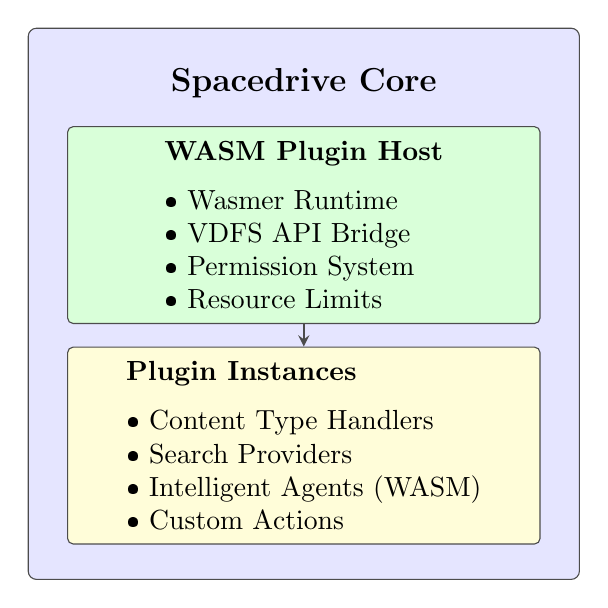
\begin{tikzpicture}[
    node distance=1.5cm,
    % Styles
    mainbox/.style={rectangle, draw=black!70, fill=blue!10, minimum width=7cm, minimum height=7cm, align=center, rounded corners=3pt},
    hostbox/.style={rectangle, draw=black!70, fill=green!15, minimum width=6cm, minimum height=2.5cm, align=left, rounded corners=2pt},
    instancebox/.style={rectangle, draw=black!70, fill=yellow!15, minimum width=6cm, minimum height=2.5cm, align=left, rounded corners=2pt},
    arrow/.style={->, >=stealth, thick, color=black!70}
]

% Main container
\node[mainbox] (core) at (0,0) {};
\node at (0,2.8) {\textbf{\large Spacedrive Core}};

% WASM Plugin Host
\node[hostbox] (host) at (0,1) {
    \textbf{WASM Plugin Host}\\[0.2cm]
    \textbullet\ Wasmer Runtime\\
    \textbullet\ VDFS API Bridge\\
    \textbullet\ Permission System\\
    \textbullet\ Resource Limits
};

% Plugin Instances
\node[instancebox] (instances) at (0,-1.8) {
    \textbf{Plugin Instances}\\[0.2cm]
    \textbullet\ Content Type Handlers\\
    \textbullet\ Search Providers\\
    \textbullet\ Intelligent Agents (WASM)\\
    \textbullet\ Custom Actions
};

% Arrow between boxes
\draw[arrow] (host.south) -- (instances.north);

\end{tikzpicture}
\caption{Spacedrive Core WASM Plugin Architecture: Sandboxed execution environment with unified API for all extension types.}
\label{fig:plugin-architecture}
\end{figure}

This architecture provides:
\begin{itemize}
    \item Complete sandboxing for all extensions
    \item Unified API for all plugin types
    \item Hot-reload capability for development
    \item Platform-independent distribution
\end{itemize}

\paragraph{Cloud Storage Integration}
Cloud storage providers (S3, Google Drive, Dropbox, etc.) are implemented as WASM plugins that leverage the OpenDAL library. This approach:
\begin{itemize}
    \item Maintains security through WASM sandboxing
    \item Enables hot-swappable cloud provider support
    \item Allows community-contributed storage backends
    \item Provides consistent API across all storage types
\end{itemize}

\subsection{Extensibility Beyond Storage: Data Ingestion Agents}
\label{sec:data-ingestion-agents}

While the VDFS architecture excels at unifying existing filesystems and storage protocols, its extensibility model enables a far more profound capability: the ingestion of disparate data from third-party services
through specialized \textbf{Data Ingestion Agents}. This transforms Spacedrive from a system that merely organizes a user's files into a comprehensive, private warehouse for their entire digital life.

These agents are lightweight, sandboxed WASM plugins that act as connectors to external data sources—social media archives, note-taking applications, code repositories, fitness trackers, and more. They leverage the
core VDFS abstractions to represent external data as native Spacedrive objects, seamlessly integrating it into the user's library.


\paragraph{Example Use Cases: A Unified Digital Life}
The potential applications create a powerful, interconnected data ecosystem:

\begin{itemize}[noitemsep, topsep=0pt]
    \item \textbf{Social Media Archiver}: An agent for Twitter could import a user's entire tweet history. Each tweet becomes an \texttt{Entry}, its text content indexed for search, and its metadata (likes, retweets)
stored in a sidecar.

    \item \textbf{Note-Taking Connector}: A Notion or Evernote agent could sync all notes into the VDFS. This would allow a user to create links between a specific note and a set of project files stored locally,
bridging the gap between knowledge management and file management.

    \item \textbf{Location Tracker}: An agent connected to a location tracking service could ingest a user's location history. The AI could then use this data to automatically tag photos and videos with the location
where they were captured.

    \item \textbf{Data-Driven Mini-Apps}: The architecture supports the creation of entire applications that use Spacedrive as their private, cross-device backend. A time-tracking app, for instance, could store all its
data directly within the user's Spacedrive Library, gaining automatic synchronization and AI capabilities for free.
\end{itemize}

This model fosters an ecosystem of "mini-apps" that offload the hard problems of storage, synchronization, and intelligence to the Spacedrive core. It fulfills the ultimate vision of the VDFS: to provide a single,
private, and intelligent foundation for a user's entire digital existence, far beyond the boundaries of the traditional filesystem.





% --- SECTION 8: SECURITY AND PRIVACY MODEL ---
\section{Security and Privacy Model}

\begin{keytakeaways}
\begin{itemize}[noitemsep, topsep=0pt]
\item \textbf{Defense in Depth}: SQLCipher database encryption + ChaCha20 network keys + TLS 1.3 transport = multi-layered protection
\item \textbf{Battle-Tested Security}: Protection against real attacks: NAS compromise, stolen devices, cloud breaches, and insider threats
\end{itemize}
\end{keytakeaways}

Spacedrive's architecture prioritizes user privacy and data security through end-to-end encryption, secure credential management, and a well-defined threat model designed for personal data scenarios.

\subsection{Data Protection at Rest}
All sensitive user data is encrypted using industry-standard cryptographic protocols:

\subsubsection{Library Database Encryption}
Each `.sdlibrary` directory employs transparent database encryption:

Library databases employ SQLCipher for transparent encryption at rest. Encryption keys are derived from user passwords using PBKDF2 with 100,000+ iterations and unique per-library salts. The unlocking process involves reading the salt, deriving the key, opening the encrypted database connection, and verifying access through a test query.

\textbf{Key derivation}: User passwords are strengthened using PBKDF2 with 100,000+ iterations and unique salts per library, providing strong protection against brute-force attacks.

\subsubsection{Network Identity Protection}
Device cryptographic keys are stored encrypted in the enhanced device configuration:

Network identity protection employs a layered approach: Ed25519 private keys are encrypted using ChaCha20-Poly1305 with keys derived through Argon2id from user passwords. Public keys remain in plaintext for identity verification. Decryption involves deriving the key using Argon2id parameters and salt, then decrypting the private key data.

\subsection{Network Security}
All network communications employ end-to-end encryption with perfect forward secrecy:

\subsubsection{Iroh QUIC Transport Security}
The Iroh networking stack provides multiple layers of security through secure connections that combine long-term device identity (Ed25519) with ephemeral session keys. Connection establishment involves a three-phase process: QUIC handshake with TLS 1.3, mutual device identity verification, and application-level key exchange for perfect forward secrecy.

\textbf{Transport Layer Security}: QUIC provides TLS 1.3 encryption for all network traffic, ensuring confidentiality and integrity.

\textbf{Application Layer Security}: Additional encryption using ephemeral keys provides perfect forward secrecy---compromising long-term device keys cannot decrypt past communications. This is particularly important for Spacedrop transfers, where each session uses completely ephemeral ECDH key exchange, ensuring that even if device keys are later compromised, past file transfers remain secure.

\subsection{Credential Management}
Spacedrive employs a secure credential storage system for cloud service integration:


\textbf{Secure Credential Vault Architecture}

Spacedrive implements a multi-layered credential protection system for cloud service integration:

\textbf{Master Key Derivation}
\begin{itemize}[noitemsep, topsep=0pt]
 \item User password transformed into cryptographically strong master key using PBKDF2
 \item Unique salt per credential vault prevents rainbow table attacks
 \item Key stretching with 100,000+ iterations provides brute-force resistance
\end{itemize}

\textbf{Individual Credential Protection}
\begin{itemize}[noitemsep, topsep=0pt]
 \item Each credential encrypted separately using ChaCha20-Poly1305 authenticated encryption
 \item Unique random nonce for each encryption operation ensures semantic security
 \item Detailed metadata tracking: service name, creation time, last access
\end{itemize}

\textbf{Storage and Lifecycle Management}
\begin{itemize}[noitemsep, topsep=0pt]
 \item Encrypted credentials stored in secure key-value mapping by service name
 \item Automatic timestamp tracking for security auditing and credential rotation
 \item Zero plaintext credential storage---everything encrypted at rest
\end{itemize}


\textbf{Platform Integration}: On supported platforms (macOS Keychain, Windows Credential Manager, Linux Secret Service), credentials are additionally protected by the OS credential store.

\subsection{Threat Model}
Spacedrive's security design addresses the following threat scenarios:

\subsubsection{Local Device Compromise}
\textbf{Threat}: Unauthorized physical access to user device.

\textbf{Mitigation}:
- Database encryption renders `.sdlibrary` directories unreadable without password
- Network keys encrypted separately, requiring password for decryption
- No plaintext credentials stored on disk

\subsubsection{Network Eavesdropping}
\textbf{Threat}: Passive monitoring of network communications.

\textbf{Mitigation}:
- All communications encrypted with TLS 1.3 via QUIC
- Perfect forward secrecy prevents retroactive decryption
- Device fingerprints prevent MITM attacks during pairing

\subsubsection{Cloud Service Compromise}
\textbf{Threat}: Breach of connected cloud storage providers.

\textbf{Mitigation}:
- Spacedrive never stores user data in cloud services---only metadata indices
- Cloud credentials encrypted locally, not shared with Spacedrive services
- Content addressing enables detection of tampered files

\subsubsection{Malicious Spacedrive Instance}
\textbf{Threat}: Compromised or malicious Spacedrive installation.

\textbf{Mitigation}:
- Libraries are portable and can be moved between trusted installations
- Audit logs provide complete history of all operations
- Action preview system prevents unauthorized operations

\subsubsection{Practical Attack Scenarios}
To illustrate the robustness of Spacedrive's security model, consider these realistic attack scenarios:

\textbf{Scenario 1: NAS Compromise and File Replacement}

\emph{Attack}: An attacker gains access to a user's NAS and replaces legitimate files with malicious versions, attempting to propagate malware across the user's device ecosystem.

\emph{Spacedrive Defense}:
\begin{itemize}[noitemsep, topsep=0pt]
\item Content addressing via BLAKE3 hashes immediately detects file modifications---the replaced files will have different hashes than the indexed versions
\item The integrity verification system flags discrepancies during the next scan, alerting the user to potential tampering
\item Version history tracking shows the exact timestamp of unauthorized modifications
\item Quarantine mechanisms prevent automatic synchronization of suspicious files to other devices
\item The audit log creates a forensic trail showing which files were modified and when
\end{itemize}

\textbf{Scenario 2: Stolen Laptop with Sensitive Photo Library}

\emph{Attack}: A laptop containing a Spacedrive library with sensitive personal photos is stolen. The attacker attempts to access the photo collection and extract metadata about locations and people.

\emph{Spacedrive Defense}:
\begin{itemize}[noitemsep, topsep=0pt]
\item SQLCipher encryption on the library database prevents access without the user's password
\item Photo metadata and AI-generated embeddings remain encrypted at rest
\item Even with physical disk access, the attacker cannot:
  - View photo thumbnails (encrypted in cache)
  - Access location data from EXIF metadata (encrypted in database)
  - Extract face recognition data or object detection results (encrypted embeddings)
\item The 100,000+ iteration PBKDF2 key derivation makes brute-force attacks computationally infeasible
\end{itemize}

\textbf{Scenario 3: Compromised Cloud Storage Credentials}

\emph{Attack}: An attacker obtains a user's cloud storage credentials through a phishing attack and attempts to inject malicious files into the user's Spacedrive-managed cloud volumes.

\emph{Spacedrive Defense}:
\begin{itemize}[noitemsep, topsep=0pt]
\item Spacedrive's credential vault remains secure---the attacker only has cloud credentials, not the Spacedrive master password
\item Content validation during cloud synchronization detects unexpected file additions
\item The volume classification system isolates cloud storage from local trusted volumes
\item File injection attempts are logged in the audit system with source attribution
\item Users can revoke cloud volume access instantly without affecting local data
\item Optional two-factor authentication on cloud volume operations provides additional protection
\end{itemize}

\textbf{Scenario 4: Insider Threat in Collaborative Team}

\emph{Attack}: A disgruntled employee on a design team attempts to exfiltrate proprietary assets and delete project files before leaving the company.

\emph{Spacedrive Defense}:
\begin{itemize}[noitemsep, topsep=0pt]
\item RBAC system restricts the employee to their assigned role permissions---they may have "Contributor" access allowing edits but not bulk deletions
\item The Action System's preview capability flags suspicious bulk operations for administrative review
\item Every file access and operation is logged in the immutable audit trail with full attribution (user, device, timestamp)
\item Data Loss Prevention (DLP) policies can detect and block unusual download patterns or transfers to external devices
\item Time-based access controls automatically revoke permissions at employment end date
\item The planned undo capability would allow administrators to instantly reverse any destructive actions
\item Cryptographic device attestation ensures actions can only originate from company-managed devices
\end{itemize}

\textbf{Scenario 5: Supply Chain Attack on Enterprise Deployment}

\emph{Attack}: An attacker attempts to compromise an enterprise Spacedrive deployment by injecting malicious code into a third-party integration or storage driver.

\emph{Spacedrive Defense}:
\begin{itemize}[noitemsep, topsep=0pt]
\item Containerized deployment isolates each component with strict network policies
\item All actions flow through the centralized Action System, preventing direct database manipulation
\item Cryptographic signatures on all deployed components ensure integrity
\item The audit system's append-only design prevents log tampering to hide malicious activity
\item Storage abstraction layer validates all operations against expected patterns
\item Regular security scanning of container images and dependencies
\item Option for air-gapped deployment in high-security environments
\end{itemize}

\subsection{Certificate Pinning and API Security}
\subsubsection{Cloud Provider Certificate Pinning}
Spacedrive implements robust certificate pinning for all cloud storage provider connections:

\textbf{Implementation Strategy}:
\begin{itemize}[noitemsep, topsep=0pt]
\item Pin both leaf certificates and intermediate CA certificates for major providers
\item Maintain backup pins for certificate rotation scenarios
\item Implement graceful fallback with user notification if pins fail
\item Regular updates through secure channels for pin refreshes
\end{itemize}

\textbf{Provider-Specific Handling}:
\begin{itemize}[noitemsep, topsep=0pt]
\item \textbf{Google Drive}: Pin GTS root and intermediate certificates
\item \textbf{Dropbox}: Pin DigiCert certificates with rotation monitoring
\item \textbf{OneDrive}: Pin Microsoft PKI infrastructure certificates
\item \textbf{S3-Compatible}: User-configurable pins for self-hosted instances
\end{itemize}

\subsection{Rate Limiting and Abuse Prevention}
\subsubsection{Multi-Layer Rate Limiting Architecture}
Spacedrive implements intelligent rate limiting to prevent abuse while maintaining performance:

\textbf{API Rate Limiting}:
\begin{itemize}[noitemsep, topsep=0pt]
\item Per-device token bucket algorithm with configurable rates
\item Separate limits for read operations (1000/min) and write operations (100/min)
\item Exponential backoff for repeated limit violations
\item Priority queuing for critical operations during limit conditions
\end{itemize}

\textbf{Network-Level Protection}:
\begin{itemize}[noitemsep, topsep=0pt]
\item Connection rate limiting per IP address (10 new connections/minute)
\item Bandwidth throttling for suspected abuse patterns
\item Automatic blacklisting for persistent violators
\item DDoS mitigation through connection pooling limits
\end{itemize}

\textbf{Operation-Level Safeguards}:
\begin{itemize}[noitemsep, topsep=0pt]
\item Bulk operation limits (max 1000 files per action)
\item Concurrent job restrictions based on device capabilities
\item Smart scheduling to prevent resource exhaustion
\item User-configurable limits for shared libraries
\end{itemize}

\subsection{Audit Log System}
The audit log system provides comprehensive tracking of user actions across all devices:

\textbf{Action Tracking}:
\begin{itemize}[noitemsep, topsep=0pt]
\item Each action creates a detailed audit entry
\item Cross-device synchronization of audit logs
\item Sequence-based ordering for chronological integrity
\item Export capability for external audit systems
\end{itemize}

\textbf{Implementation Details}:
\begin{lstlisting}[language=Rust, caption={Audit log entry structure}]
pub struct AuditEntry {
    pub id: Uuid,
    pub timestamp: DateTime<Utc>,
    pub action: ActionType,
    pub device_id: DeviceId,
    pub details: serde_json::Value,
    pub sequence_number: u64,
}

impl AuditEntry {
    pub fn new(action: ActionType, device_id: DeviceId) -> Self {
        Self {
            id: Uuid::new_v4(),
            timestamp: Utc::now(),
            action,
            device_id,
            details: serde_json::Value::Null,
            sequence_number: 0, // Assigned during sync
        }
    }
}
\end{lstlisting}

\textbf{Sync Integration}:
\begin{itemize}[noitemsep, topsep=0pt]
\item Audit logs sync as UserMetadata across devices
\item Sequence numbers ensure proper ordering
\item Conflict resolution preserves all audit entries
\item Background reconciliation maintains consistency
\end{itemize}

\subsection{Spacedrive Cloud Service Privacy Model}
The managed Spacedrive Cloud Service treats privacy as a fundamental design principle, not an afterthought:

\subsubsection{End-to-End Encryption Architecture}
The Cloud Core instance runs the standard Spacedrive software with no special privileges or backdoors:

\textbf{Cryptographic Isolation}:
\begin{itemize}[noitemsep, topsep=0pt]
 \item Each Cloud Core runs in an isolated container with unique cryptographic identity
 \item Network policies enforce that only paired devices can communicate
 \item No shared infrastructure between different user instances
 \item Complete data isolation at storage, network, and compute layers
 \item Data is encrypted in transit and at rest
\end{itemize}

\subsubsection{Operational Security}
Infrastructure access is strictly controlled and audited:

\textbf{Administrative Access}:
\begin{itemize}[noitemsep, topsep=0pt]
 \item No direct access to user containers or data volumes
 \item Administrative operations limited to resource management and health monitoring
 \item All infrastructure access logged and audited
 \item User data remains encrypted even during backup operations
\end{itemize}

\textbf{Data Retention and Deletion}:
\begin{itemize}[noitemsep, topsep=0pt]
 \item User data is permanently deleted within 30 days of account closure
 \item Cryptographic erasure ensures data cannot be recovered
 \item Users can export their entire library before deletion
 \item No data mining or analysis of user content
\end{itemize}

\subsection{Privacy-Preserving AI}
The AI-native architecture maintains privacy through multiple mechanisms:


\textbf{Flexible AI Provider Selection for Privacy Control}

Spacedrive supports multiple AI deployment models to balance privacy, performance, and capability:

\textbf{Local AI Processing (Maximum Privacy)}
\begin{itemize}[noitemsep, topsep=0pt]
 \item Integrates with Ollama for completely local AI model execution
 \item User data never leaves the device---complete privacy preservation
 \item Configurable endpoint and model selection for different AI capabilities
 \item Works offline once models are downloaded
\end{itemize}

\textbf{Self-Hosted Solutions (Organizational Control)}
\begin{itemize}[noitemsep, topsep=0pt]
 \item Custom AI infrastructure under user or organization control
 \item Flexible authentication options for enterprise deployment
 \item Complete control over data processing and model selection
 \item Ideal for organizations with specific privacy or compliance requirements
\end{itemize}

\textbf{Cloud AI Services (Enhanced Capabilities)}
\begin{itemize}[noitemsep, topsep=0pt]
 \item Access to state-of-the-art models from major AI providers
 \item Encrypted API key storage with detailed privacy policy tracking
 \item Transparent data processing terms presented to users for informed consent
 \item Metadata-only transmission---file contents remain local
\end{itemize}


\textbf{Local Processing}: Default to local AI models (Ollama) that never transmit user data externally.

\textbf{Metadata-Only Cloud Processing}: When using cloud AI services, only file metadata (names, types, sizes) are transmitted---never file contents.

\textbf{User Control}: Complete transparency about which AI provider processes which data, with granular user control over privacy vs. capability trade-offs.

\subsection{Balancing Privacy and Public Sharing}

Spacedrive's security model accommodates both zero-knowledge privacy and public content sharing through its library-based architecture.

\subsubsection{Per-Library Encryption Policy}

Each library maintains independent encryption settings:

\begin{itemize}
    \item \textbf{Private Libraries} (default): Full SQLCipher encryption at rest
    \item \textbf{Public Libraries} (opt-in): Unencrypted for web serving
    \item \textbf{Hybrid Libraries}: Encrypted with selective public locations
\end{itemize}

\begin{lstlisting}[language=Rust, caption=Library encryption configuration]
pub struct LibraryConfig {
    pub encryption: EncryptionMode,
    pub public_sharing: PublicSharingConfig,
}

pub enum EncryptionMode {
    /// Full encryption (default)
    Encrypted { key_derivation: Argon2id },
    /// No encryption (for public content)
    Unencrypted,
    /// Encrypted with public locations
    Hybrid { public_locations: Vec<LocationId> },
}

pub struct PublicSharingConfig {
    /// Which core serves public content
    pub hosting_core: CoreIdentity,
    /// Custom domain (if any)
    pub custom_domain: Option<String>,
    /// Access control rules
    pub access_rules: Vec<AccessRule>,
}
\end{lstlisting}

\subsubsection{Secure Public Sharing Workflow}

Users can share content publicly without compromising private data:

\begin{enumerate}
    \item Create a dedicated public library or location
    \item Configure which core hosts public content (cloud or self-hosted)
    \item Move/copy files to public locations
    \item Share generated URLs with recipients
    \item Private libraries remain fully encrypted throughout
\end{enumerate}

\subsubsection{Implementation Considerations}

This dual-mode approach ensures:

\begin{itemize}
    \item \textbf{Clear Boundaries}: Users explicitly choose what becomes public
    \item \textbf{No Encryption Downgrade}: Private libraries cannot be converted to public
    \item \textbf{Audit Trail}: All public sharing actions are logged
    \item \textbf{Revocable Access}: Public files can be made private instantly
    \item \textbf{Hosting Flexibility}: Any core can serve public content with proper setup
\end{itemize}

\paragraph{Security Implications}
The system maintains security through isolation:

\begin{itemize}
    \item Public and private data never mix within a library
    \item Encryption keys are never exposed to hosting infrastructure
    \item Access tokens are scoped to specific libraries and operations
    \item Public URLs use capability-based security (unguessable paths)
\end{itemize}

By making encryption optional but enabled by default, Spacedrive provides flexibility for content creators and enterprises while maintaining strong privacy guarantees for personal data.





% --- SECTION 10: CONCLUSION ---
\section{Conclusion}

\begin{keytakeaways}
\begin{itemize}[noitemsep, topsep=0pt]
\item \textbf{Accessible Design}: Enterprise-grade distributed file management for all users
\item \textbf{Production Proven}: Real implementation handling millions of files with sub-100ms response times validates every architectural decision
\item \textbf{Future Ready}: Solid foundation for AI agents, federated learning, and evolving human-computer interaction
\end{itemize}
\end{keytakeaways}

Spacedrive rethinks personal file management by making distributed systems capabilities accessible to individual users. Through our implementation, we have shown that personal data management can evolve beyond simple file browsers to become intelligent, distributed systems that respect user ownership while providing enterprise-level capabilities, embodying the principles of local-first software~\cite{kleppmann_localfirst_2019} and ubiquitous computing~\cite{weiser_ubiquitous_1991}.

\subsection{Key Contributions and Real-World Impact}
This work transforms personal file management through five innovations: AI-native natural language operations, universal cross-device file addressing, immediate metadata for every file, domain-separated synchronization, and performance-aware deduplication.

The impact is practical. Users manage millions of files across dozens of devices through a single interface, eliminating storage waste while maintaining sub-second response times. Data remains portable, privacy is preserved through local-first design, and AI enhancement comes without sacrificing user control. Our Rust implementation validates these concepts at scale.

\subsection{System Integration}
These innovations work together to create powerful combined capabilities. The Library abstraction makes backup and migration trivial (copy a directory), while SdPath enables seamless operations across that distributed storage. Content addressing works transparently with the sync system to maintain deduplication relationships even as files move between devices. The Temporal-Semantic Search architecture leverages both the content addressing and metadata systems to provide semantic discovery at traditional keyword search speeds.

\subsection{Validation in Production}
Spacedrive's architecture has been validated through production implementation in Rust, demonstrating that these concepts work reliably in practice. The system handles millions of files across multiple devices while maintaining sub-second response times for user operations. The extensive test framework, including multi-process distributed testing, ensures that the complex interactions between networking, synchronization, and file operations remain stable across diverse deployment scenarios.

\subsection{Future Work and Roadmap}
The architectural foundation laid by Spacedrive opens concrete paths for near-term enhancements and long-term research directions. Our immediate roadmap focuses on extending the AI capabilities to support complex multi-step workflows, such as "organize all vacation photos by year and location, then create albums for each trip." This involves expanding the Action system to support workflow composition while maintaining the same security and reversibility guarantees. Parallel to this, we are developing intelligent content analysis pipelines that leverage both local and cloud models to automatically extract semantic information from files---identifying people in photos, extracting key topics from documents, and understanding relationships between files based on content rather than just metadata. The existing FFmpeg integration provides a foundation for planned media processing capabilities including on-demand transcoding, format conversion, and adaptive streaming support for seamless media playback across devices.

In the medium term, our research agenda includes three major initiatives. First, we are exploring federated learning approaches that would allow users to benefit from collective intelligence about file organization patterns while maintaining complete privacy---the system would learn from aggregate behaviors without ever exposing individual file information. Second, we are developing advanced storage tiering algorithms that combine AI predictions with real-time access patterns to automatically move files between fast local storage, slower archives, and cloud services based on predicted access likelihood and user-defined cost constraints. Third, we are investigating cross-Library content discovery mechanisms that would allow users to identify duplicate content across different Libraries (perhaps owned by family members or team members) while maintaining the strong isolation guarantees that make Libraries portable and secure. Additionally, we are expanding protocol support via community plugins, enabling deeper integration with enterprise storage systems like SMB/NFS and emerging decentralized protocols.

The longer-term vision extends Spacedrive beyond personal file management into a platform for personal AI agents that understand and manage all aspects of a user's digital life. By providing a complete, versioned view of a user's file history combined with rich semantic understanding, Spacedrive could enable AI assistants that truly understand context---not just current file state but how information has evolved over time. This temporal understanding, combined with the robust Action system, would allow AI agents to perform complex organizational tasks with confidence, knowing that all actions are reversible and auditable. The architecture's emphasis on user control ensures that as these AI capabilities grow more sophisticated, users retain ultimate authority over their data, with all AI operations remaining transparent, explainable, and reversible.

\subsection{Limitations}
While Spacedrive advances personal data management, it has boundaries. The single-device database model limits scalability beyond 100M files without sharding, potentially constraining extreme enterprise use. Mobile resource constraints may delay background indexing on low-power devices. The AI layer, while privacy-focused, requires capable hardware for local models, and cloud alternatives introduce latency. Finally, while offline-first, initial setup requires internet for device pairing in distributed scenarios.

These limitations inform our roadmap, ensuring future iterations maintain core principles while expanding capabilities.

\subsection{Broader Implications}
Spacedrive shows that user-centric applications can also be powerful enterprise systems. Through careful domain separation, a local-first security model, and an architecture built for scale, we have demonstrated that it is possible to build a single platform that serves the needs of both individual users and large organizations. The key insight is that by starting with a foundation of user empowerment and data sovereignty, we create a system that naturally scales up to enterprise requirements while maintaining the simplicity and control that individual users demand.

This approach suggests a path forward for personal computing that moves beyond the current model of data scattered across incompatible cloud services toward truly user-controlled, portable, and intelligent data management. The native cloud service model presented in Section 5 is a clear manifestation of this principle, proving that cloud convenience does not have to come at the cost of architectural integrity or user control. By treating the cloud as just another trusted peer, Spacedrive offers a viable hybrid model for the future of personal data. By treating personal data as a unified library rather than a collection of disconnected files, users gain both the simplicity of traditional file management and the power of modern distributed systems.

Spacedrive's architecture provides a robust foundation for the next generation of computing---one that bridges personal and enterprise needs seamlessly. Whether serving an individual creator, a small team, or a global enterprise, the platform delivers the same core promise: unified access to all data, intelligent assistance without sacrificing control, and a user experience that makes powerful capabilities feel effortless. This provides a new approach for how users and organizations interact with their digital assets at any scale.

We invite researchers, developers, and users to contribute to Spacedrive's open-source ecosystem at \url{https://github.com/spacedriveapp/spacedrive}, advancing the future of personal data management.


% --- ACKNOWLEDGMENTS ---
\begin{acks}
We thank the open-source community, particularly the developers of the Rust programming language and its ecosystem, including the Tauri, Iroh, Tokio and SeaORM projects, whose work provided the foundation for this research.

The authors acknowledge the use of generative AI tools for assistance in drafting and refining the prose of this whitepaper. The core architectural concepts, technical details, and design are the original work of the authors, who take full responsibility for the content and accuracy of this paper.
\end{acks}


% --- GLOSSARY ---
\appendix
\section{Glossary of Terms}

\subsection*{Core Concepts}

\textbf{Action}: A pre-visualized, durable file operation that can be simulated before execution. Actions are the primary way users interact with files in Spacedrive.

\textbf{CAS (Content-Addressed Storage)}: A storage system where data is identified by its content hash rather than location, enabling automatic deduplication.

\textbf{Entry}: The fundamental data unit in Spacedrive representing any filesystem entity (file or directory) with immediate metadata capabilities.

\textbf{Library}: A portable, self-contained \texttt{.sdlibrary} directory containing a complete Spacedrive database, configuration, and metadata for a user's data ecosystem.

\textbf{Temporal-Semantic Search}: Spacedrive's two-stage hybrid search architecture combining temporal-first filtering with vector-enhanced semantic discovery.

\textbf{SdPath}: Spacedrive's universal path abstraction that transparently addresses files across devices, volumes, and cloud storage.

\textbf{VDFS (Virtual Distributed File System)}: A unified index of all user data across devices while keeping files in their original locations.

\subsection*{Technical Components}

\textbf{Content Identity}: A unique identifier based on file content hash that tracks all instances of identical content across the Library.

\textbf{CRDT (Conflict-free Replicated Data Type)}: A data structure that automatically resolves conflicts in distributed systems. Note: Spacedrive v1 attempted a custom CRDT implementation that proved overly complex. V2 replaced this with a simpler domain separation approach (see Section~\ref{sec:library-sync}).

\textbf{FTS (Full-Text Search)}: Traditional keyword-based search capability integrated into Spacedrive's Temporal-Semantic Search system.

\textbf{Phantom Path}: A special SdPath variant representing files that may not currently exist but are referenced in the Library index.

\textbf{Virtual Sidecar System}: A system for managing derivative data (e.g., thumbnails, OCR text, transcripts) associated with a file Entry. These sidecar files are stored within the Spacedrive Library and linked to the original file via the VDFS index, ensuring the original file is never modified.

\textbf{Volume}: Any storage location (local drive, network mount, cloud service) that Spacedrive can access and index.

\textbf{OpenDAL}: Open Data Access Layer, providing unified access to cloud storage services.

\textbf{ContentKind}: Semantic categorization system that groups files into 17 intuitive categories (Image, Video, Code, etc.) beyond traditional MIME types.

\textbf{File Type System}: Advanced multi-method file identification combining extension matching, magic byte detection, and content analysis with confidence scoring.

\subsection*{Architecture \& Deployment}

\textbf{Daemon}: A background service that hosts the Spacedrive core engine, providing persistent state management and enabling multiple clients to connect concurrently.

\textbf{Embedded Mode}: Deployment model where the core is directly linked into the application binary, used for mobile apps and standalone distributions.

\textbf{IPC (Inter-Process Communication)}: The mechanism for client-daemon communication using Unix domain sockets or named pipes with a JSON-RPC protocol.

\textbf{WASM Plugin}: WebAssembly-based extension running in a sandboxed environment.

\textbf{Integration}: WASM plugin providing system integration (e.g., cloud storage).

\subsection*{Synchronization \& Networking}

\textbf{Library Sync}: Spacedrive's leaderless, peer-to-peer synchronization system. It uses a hybrid model: simple state-based replication for device-authoritative data (like the file index) and a lightweight, HLC-ordered log for shared metadata (like tags and collections). Each syncable model defines its own conflict resolution strategy, from implicit union merge for tag assignments to deterministic last-writer-wins for scalar values. This eliminates central coordinators and single points of failure while ensuring eventual consistency.

\textbf{Hybrid Logical Clock (HLC)}: A distributed timestamping mechanism that combines physical time with a logical counter to create a total ordering of events across multiple devices. Used in Spacedrive to deterministically resolve conflicts for shared metadata without requiring a central coordinator

\textbf{Iroh}: The peer-to-peer networking library used for device discovery and secure communication.

\textbf{P2P (Peer-to-Peer)}: Direct device-to-device communication without requiring a central server.

\textbf{RPC (Remote Procedure Call)}: The mechanism for executing operations on remote devices in the Spacedrive network.

\textbf{Spacedrop}: Spacedrive's ephemeral file sharing protocol enabling secure, AirDrop-like transfers between any devices without requiring prior pairing or trust relationships.

\subsection*{Storage \& Performance}

\textbf{Adaptive Hashing}: Strategic content sampling for large files to maintain deduplication effectiveness without full-file hashing overhead.

\textbf{Intelligent Storage Tiering}: Automatic management of hot (frequently accessed) and cold (archival) data across different storage tiers.

\textbf{Semantic Label}: User-friendly volume names (e.g., "Jamie's MacBook") that persist across device reconnections.

\textbf{StorageClass}: The effective storage tier of a file, determined by taking the more restrictive class between a Volume's \texttt{PhysicalClass} and a Location's \texttt{LogicalClass}.

\textbf{PhysicalClass}: An automatically detected property of a Volume that reflects its physical capabilities (e.g., Hot for SSD, Cold for an archival cloud tier).

\textbf{LogicalClass}: A user-defined property on a Location that reflects its intended organizational purpose (e.g., marking a folder as an archive).

\textbf{Volume Classification}: Platform-aware categorization of storage devices to optimize performance and user experience.

\subsection*{File Formats \& Standards}

\textbf{AVIF}: A modern image format used for efficient thumbnail storage.

\textbf{JSON}: JavaScript Object Notation, used for configuration and data exchange.

\textbf{BLAKE3}: The cryptographic hash function used for content addressing, chosen for its speed and security.

\textbf{SQLite}: The embedded database engine powering Spacedrive's local-first architecture.

\textbf{UUID}: Universally Unique Identifier used for device and entry identification.

\textbf{WebP}: An image format used for efficient thumbnail compression.

\subsection*{Platform Acronyms}

\textbf{API}: Application Programming Interface.

\textbf{CLI}: Command Line Interface.

\textbf{CPU}: Central Processing Unit.

\textbf{GUI}: Graphical User Interface.

\textbf{NAS}: Network Attached Storage.

\textbf{OS}: Operating System.

\textbf{SMB}: Server Message Block protocol for network file sharing.

\textbf{SQL}: Structured Query Language.

\textbf{UI}: User Interface.

\subsection*{AI-Related Terms}

\textbf{AI-Native Architecture}: Spacedrive's design philosophy where AI capabilities are foundational rather than added features.

\textbf{Ollama}: An open-source platform for running large language models locally.

\textbf{Semantic Search}: Search capability that understands meaning and context rather than just matching keywords.

\textbf{Vector Search}: Search using mathematical representations of content meaning for semantic similarity matching.


% --- REFERENCES ---
\bibliographystyle{ACM-Reference-Format}
\bibliography{references}

\end{document}
